% =====================================================================================
% P2 - Finanças do Setor Público (UnB, CCA0169, 2026.2) - Artigo
% Compilar no Overleaf com pdfLaTeX + BibTeX (padrão). Nome do PDF final: 232045821_P2_FSP.pdf
% Estrutura: o texto de cada seção fica em secoes/; tabelas geradas por código em tabelas/;
% figuras em figuras/. Comentários com "TODO" indicam o que falta escrever.
% =====================================================================================
\documentclass[12pt,a4paper]{article}

% ---------- idioma, fonte e página
\usepackage[T1]{fontenc}
\usepackage[utf8]{inputenc}
\IfFileExists{brazil.ldf}{\usepackage[brazil]{babel}}{\usepackage[brazilian,provide=*]{babel}}
\usepackage{mathptmx}  % Times, conforme o uso da ABNT
\usepackage{microtype}
\usepackage{indentfirst}  % recuo também no primeiro parágrafo de cada seção (ABNT)
\usepackage[a4paper,top=3cm,left=3cm,bottom=2cm,right=2cm]{geometry}
\usepackage{setspace}\onehalfspacing
\setlength{\parindent}{1.25cm}

% ---------- matemática, tabelas e figuras
\usepackage{amsmath,amssymb}
\usepackage{graphicx}
\usepackage{booktabs,threeparttable,tabularx,multirow,adjustbox}
\usepackage{siunitx}
\sisetup{output-decimal-marker={,},group-separator={.},group-minimum-digits=4}
\usepackage{float}
\usepackage[font=small,labelfont=bf,justification=centering]{caption}
\usepackage{enumitem}

% ---------- citações (autor-ano) e links
\usepackage[round,authoryear]{natbib}
\usepackage[hidelinks]{hyperref}
\urlstyle{same}

% ---------- títulos das seções no tamanho do texto (ABNT)
\usepackage{titlesec}
\titleformat*{\section}{\normalsize\bfseries}
\titleformat*{\subsection}{\normalsize\bfseries}
\titlespacing*{\section}{0pt}{12pt}{6pt}
\titlespacing*{\subsection}{0pt}{12pt}{6pt}
\AtBeginDocument{\renewcommand{\contentsname}{SUMÁRIO}\renewcommand{\refname}{REFERÊNCIAS}\renewcommand{\abstractname}{RESUMO}}

% ---------- atalhos
\newcommand{\todo}[1]{\textcolor{red}{[TODO: #1]}}
\usepackage{xcolor}
\newcommand{\fonte}[1]{\par\vspace{2pt}{\footnotesize Fonte: #1}}

\begin{document}

% ========================== capa
\begin{titlepage}
\centering

\includegraphics[width=6.5cm]{figuras/logo_unb.png}\par
\vspace{1cm}
João Gabriel Maréco Galhas --- Matrícula 232045821\par
\vspace{0.3cm}
Universidade de Brasília (UnB) --- Finanças do Setor Público (CCA0169), Turma 01, 2026.2\par
Professor: Lucas Oliveira Gomes Ferreira\par
\vfill
{\bfseries Dependência de transferências, autonomia fiscal e efeito \textit{flypaper}: Barreiras e Camaçari (BA) e os governos locais da Hungria (2016--2025)\par}
\vfill
Brasília, outubro de 2026\par
\end{titlepage}

% ========================== sumário (folha sem número; a contagem segue)
\setcounter{page}{2}
\begingroup
\singlespacing
\tableofcontents
\endgroup
\thispagestyle{empty}
\clearpage

% ========================== resumo
\begin{abstract}
\noindent Este artigo discute se a dependência de transferências, indicador usado para avaliar a autonomia fiscal dos municípios brasileiros, mede o que promete. A questão nasce de uma distorção contábil: a cota-parte do ICMS é registrada como transferência do estado, embora seja repartida conforme a riqueza produzida em cada município, e por isso recebe o mesmo nome de repasses que vêm de fora, como o Fundo de Participação dos Municípios (FPM). Para examinar essa distorção, o estudo compara Barreiras e Camaçari, na Bahia, que recebem o mesmo FPM, mas têm economias opostas, e contrasta esses casos com os governos locais da Hungria, um Estado unitário que recentralizou suas finanças. A pesquisa atualiza até 2025 e corrige a base de um trabalho anterior e combina análise descritiva com regressões que testam o efeito \textit{flypaper}, segundo o qual o gasto local reage mais às transferências do que à renda dos moradores. Os resultados mostram que o indicador convencional ordena corretamente os dois municípios, mas superestima a dependência de Camaçari: sem a cota do ICMS gerada por sua indústria, a parcela de sua receita que vem de fora cai, em média, de 61\% para 27\%. Na Hungria, a dependência caiu enquanto os governos locais perdiam competências. Já o teste do \textit{flypaper} não consegue separar a resposta do gasto às transferências da simples regra de gastar o que se arrecada. Ao expor os limites dessa medida, o artigo contribui para avaliar melhor a autonomia municipal, às vésperas da substituição do ICMS pela reforma tributária, e oferece uma base de dados aberta e reprodutível.

\vspace{0.5em}
\noindent\textbf{Palavras-chave:} transferências intergovernamentais; efeito \textit{flypaper}; ilusão fiscal; autonomia fiscal; cota-parte do ICMS; Hungria.\\
\noindent\textbf{Classificação JEL:} H71; H72; H77.\\
\noindent\textbf{Dados e códigos:} \url{https://github.com/joaogabrielmarecogalhas9154-blip/P2-FSP-232045821}
\end{abstract}


% ========================== corpo
\section{INTRODUÇÃO}\label{sec:introducao}

Este estudo analisa como o federalismo fiscal brasileiro, ao repassar aos municípios recursos da União, por meio do FPM, e dos estados, por meio da cota-parte do ICMS, pode distorcer a leitura de quanto cada um depende, de fato, de recursos de fora. Nesse escopo, foram analisados dois municípios da Bahia: Barreiras, no oeste baiano, e Camaçari, na Região Metropolitana de Salvador. Os dois recebem exatamente o mesmo valor do FPM desde 2018, R\$~214,1 milhões cada um em 2025, mas têm economias opostas: Camaçari é sede de um polo industrial, e Barreiras vive dos serviços regionais e da agropecuária. Em Barreiras, as transferências financiam cerca de 80\% da receita corrente; em Camaçari, entre 56\% e 65\%. O estudo compara ainda esses casos com a Hungria, que, diferentemente do Brasil, é um Estado unitário e não garante aos governos locais fatias automáticas da arrecadação nacional.

Esse contraste interessa às finanças públicas porque toca dois problemas clássicos do federalismo fiscal. O primeiro é o efeito \textit{flypaper}. Pelo modelo do eleitor mediano, uma transferência incondicional deveria elevar o gasto local tanto quanto um aumento equivalente na renda dos moradores; na prática, eleva muito mais \citep{HinesThaler1995}. O segundo é a ilusão fiscal: quando parte do custo dos serviços é paga por terceiros ou por tributos pouco visíveis, os contribuintes subestimam esse custo e passam a demandar mais gasto \citep{DolleryWorthington1996}. A tese que serve de referência a este trabalho trata o primeiro fenômeno como uma forma do segundo. Ela encontra o efeito em estados e municípios brasileiros, mais forte onde é mais custoso arrecadar com tributos locais, o chamado custo marginal dos fundos públicos \citep{Ferreira2021}.

As duas ideias dependem de uma separação simples: o que é receita gerada pela economia local e o que é dinheiro vindo de fora. A contabilidade pública brasileira mistura as duas coisas. A cota-parte do ICMS é registrada como transferência do estado, mas pelo menos 65\% dela é repartida conforme o valor adicionado em cada município \citep{CF1988art158}. Num município industrial, essa ``transferência'' sobe e desce com a atividade das próprias empresas; num município sem base produtiva relevante, funciona como um repasse redistributivo. Mesmo assim, a contabilidade dá às duas situações o mesmo nome: dependência de transferências. A distinção não é nova: a OCDE já separa quem controla a receita de quem a gera \citep{BlochligerKing2006}, e o Índice de Autonomia Local mede à parte o poder de tributar e conta a parcela incondicional dos repasses como autonomia de gasto \citep{Ladner2016}. O que este artigo examina são suas consequências em dois municípios que recebem exatamente o mesmo FPM.

O \textit{flypaper} e a ilusão fiscal ajudam a entender por que as transferências podem desestimular a arrecadação própria e esconder do eleitor o custo dos serviços. Há, porém, um passo anterior: saber o que é, de fato, transferência. Parte da renda gerada no município é tributada pelo estado e volta a ele como cota do ICMS, na proporção do que ali se produziu; outra parte da receita, como o FPM, vem da arrecadação nacional e é repartida pela população. A contabilidade trata as duas como dependência. O artigo pergunta, então, \textit{em que medida as transferências incondicionais se associam ao gasto de Barreiras e Camaçari mais do que a renda local, e como a dependência desses municípios se compara à dos governos locais da Hungria}. Sustenta-se que a dependência, como a contabilidade a registra, não acompanha a autonomia fiscal. No Brasil, ela ordena corretamente os municípios, mas superestima a dependência de recursos externos de quem tem a receita vinculada à própria economia; na Hungria, caiu enquanto os governos locais perdiam competências. Na parte econométrica, o gasto acompanha as transferências mais do que o PIB, mas, com dois municípios, não é possível separar esse padrão do ciclo comum das receitas.

A Hungria, segundo caso do estudo, percorreu o caminho inverso. A partir de 2011, com a nova Constituição e a nova lei de governos locais, o país recentralizou suas finanças locais em duas ondas \citep{Dobos2025}. Na primeira, o Estado assumiu as escolas, ao fim de 2012 \citep{Semjen2023}, e as dívidas acumuladas pelos municípios \citep{Vasvari2020571}. Desde 2013, passou também a financiar tarefas específicas com recursos carimbados, em vez de repartir receitas \citep{OCDE_UCLG2016}. Na segunda onda, a partir de 2019, os recursos discricionários passaram a favorecer prefeituras alinhadas ao governo e a faltar às de oposição \citep{Vasvari2024467, Kovarek2023}. Ao mesmo tempo, a contribuição de solidariedade, criada em 2017, passou a recolher ao orçamento nacional uma parte crescente do imposto local dos municípios que mais arrecadam \citep{CoE2024}. O resultado mostra o limite do indicador: os governos locais encolheram de 9,2\% para 5,4\% do PIB entre 2012 e 2025 e perderam poder, mas o peso das transferências em sua receita caiu. Pelo indicador usual, pareceriam mais autônomos. A comparação serve, portanto, para ver se a medida de dependência diz a verdade nos dois sentidos, e não para confrontar números de dois países: a lição húngara está menos no modelo unitário do que no indicador.

Para responder à pergunta, o artigo atualiza e corrige a base de dados do trabalho anterior sobre os mesmos casos \citep{DutraP1}, estendendo-a até 2025; compara a composição das receitas dos dois municípios; e estima a relação entre gasto, transferências e PIB, com testes de robustez. A principal contribuição é mostrar, com uma base corrigida e reprodutível, que, sob o mesmo FPM, o indicador convencional mais que dobra a dependência de recursos externos do município industrial, porque conta como transferência a receita gerada por sua própria indústria. A análise descritiva cobre de 2016 a 2025; as regressões vão de 2014 a 2023, último ano com PIB municipal. A Seção~\ref{sec:referencial} discute a literatura e apresenta o panorama bibliométrico; a Seção~\ref{sec:metodologia} descreve dados e métodos; a Seção~\ref{sec:resultados} apresenta os resultados; e a Seção~\ref{sec:conclusao} conclui.

\section{REFERENCIAL TEÓRICO}\label{sec:referencial}

\subsection{Panorama bibliométrico da literatura}\label{sec:bibliometria}

Para dimensionar o campo e orientar a seleção das referências, realizou-se um levantamento bibliométrico na base Scopus, processado com o pacote bibliometrix \citep{AriaCuccurullo2017}, em formato inspirado na abertura de \citet{Baker2022}. A busca, feita em 22 de outubro de 2026 nos títulos, resumos e palavras-chave, usou a expressão em inglês (\textit{``flypaper effect'' OR ``fiscal illusion'' OR ``intergovernmental transfer*'' OR ``intergovernmental grant*''}) AND (\textit{municipal* OR ``local government*'' OR subnational}) e foi restrita a artigos de periódicos publicados entre 2016 e 2026. Termos como \textit{fiscal transfers}, \textit{revenue sharing} e \textit{equalization} não foram incluídos; o conjunto recuperado é, portanto, uma amostra da literatura sobre transferências a governos locais, não o seu universo.

A busca retornou 327 artigos, dos quais 54 (16,5\%) tratam especificamente de efeito \textit{flypaper} ou de ilusão fiscal, critério aplicado aos títulos, resumos e palavras-chave (Tabela~\ref{tab:bibliometria} e Figura~\ref{fig:producao}). Considerados apenas os anos completos, a produção subiu de 23 artigos por ano em 2016--2019 para 32 em 2020--2022 e ficou em 29 em 2023--2025; somados, os períodos têm 92, 97 e 138 artigos, este último com 2026 incompleto. Os artigos específicos somam 15, 20 e 19 nesses períodos, ou 16,3\%, 20,6\% e 13,8\% do total. Com contagens tão pequenas, a variação dessas participações não permite afirmar uma mudança de agenda; indica apenas que os dois conceitos ocupam uma fatia estável e minoritária de uma literatura que cresceu até 2022 e depois se estabilizou.

A distribuição por periódico mostra onde esses conceitos circulam. Os títulos que mais publicam pertencem às finanças públicas e à economia política, com destaque para \textit{Local Government Studies} e \textit{Public Finance Review}, com 11 artigos cada. Em \textit{Local Government Studies} e \textit{Lex Localis}, cerca de metade dos artigos trata de \textit{flypaper} ou de ilusão fiscal; no \textit{European Journal of Political Economy}, nenhum dos dez artigos emprega esses termos, embora alguns tratem do fenômeno, como o de \citet{Shani2023}. Os demais 247 artigos (75,5\%) dispersam-se por outros periódicos. Essa base, complementada por estudos brasileiros não indexados na Scopus e por clássicos indispensáveis, forneceu o núcleo das referências discutidas a seguir.

\IfFileExists{tabelas/tabela1_bibliometria.tex}{\begin{table}[H]
\centering\footnotesize\setlength{\tabcolsep}{5pt}
\caption{Uso dos conceitos de efeito \textit{flypaper} e ilusão fiscal na literatura sobre transferências a governos locais, por periódico (2016--2026)}
\label{tab:bibliometria}
\begin{threeparttable}
\begin{tabular}{lccc}
\toprule
 & (1) & (2) & (3) \\
 & Transferências a & \textit{Flypaper} ou & (2)/(1) \\
Periódico & governos locais & ilusão fiscal & (\%) \\
\midrule
Local Government Studies & 11 & 6 & 54,5\% \\
Public Finance Review & 11 & 3 & 27,3\% \\
European Journal of Political Economy & 10 & 0 & 0,0\% \\
International Tax and Public Finance & 10 & 1 & 10,0\% \\
Public Choice & 8 & 2 & 25,0\% \\
Public Budgeting and Finance & 7 & 1 & 14,3\% \\
Lex Localis & 6 & 3 & 50,0\% \\
Regional Studies & 6 & 0 & 0,0\% \\
World Development & 6 & 0 & 0,0\% \\
Regional Science and Urban Economics & 5 & 1 & 20,0\% \\
Demais periódicos & 247 & 37 & 15,0\% \\
\midrule
Total & 327 & 54 & 16,5\% \\
\bottomrule
\end{tabular}
\begin{tablenotes}[flushleft]\footnotesize
\item Nota: A tabela resume o número de artigos publicados em periódicos científicos entre 2016 e 2026 sobre transferências intergovernamentais a governos locais. A busca foi realizada em 22/10/2026 na base Scopus, nos campos título, resumo e palavras-chave, com a expressão: ("flypaper effect" OR "fiscal illusion" OR "intergovernmental transfer*" OR "intergovernmental grant*") AND (municipal* OR "local government*" OR subnational), restrita a artigos de periódico publicados entre 2016 e 2026. A busca retornou 327 artigos. A coluna (1) apresenta todos os artigos; a coluna (2), os que tratam especificamente de efeito flypaper ou de ilusão fiscal (termos presentes no título, no resumo ou nas palavras-chave; artigos que tratam do fenômeno sem usar esses termos ficam apenas na coluna 1); a coluna (3), a participação de (2) em (1). As linhas listam os dez periódicos com mais artigos; os demais estão agregados. Os dados de 2026 são parciais (artigos indexados até a data da busca). Processamento: pacote bibliometrix (Aria e Cuccurullo, 2017) no R.
\end{tablenotes}
\end{threeparttable}
\end{table}
}{}

\IfFileExists{figuras/figura_producao_anual.png}{%
\begin{figure}[H]
  \centering
  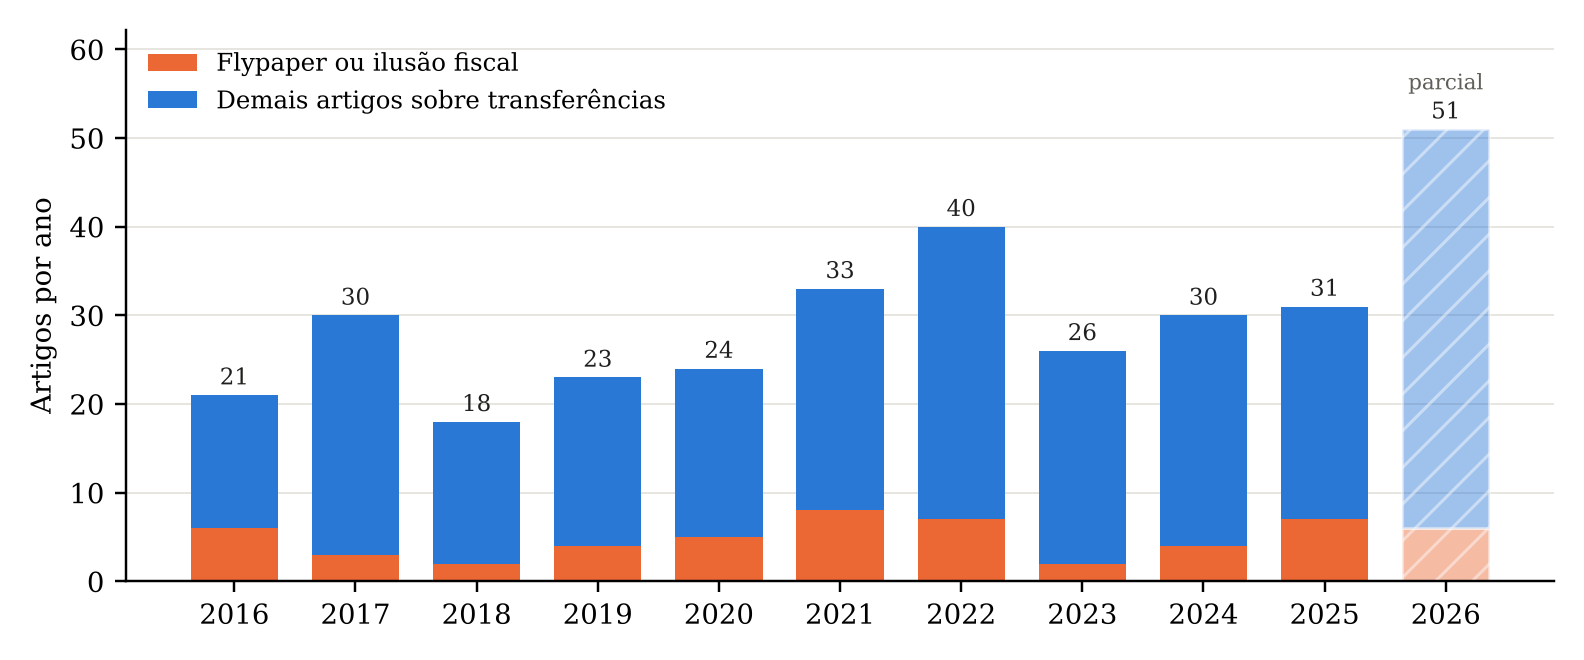
\includegraphics[width=0.9\textwidth]{figuras/figura_producao_anual.png}
  \caption{Produção anual de artigos recuperados pela busca (2016--2026): total e artigos sobre efeito \textit{flypaper} ou ilusão fiscal}
  \label{fig:producao}
  \fonte{elaboração própria a partir da base Scopus (busca em 22/10/2026), com a contagem do bibliometrix \citep{AriaCuccurullo2017}. Barras hachuradas: 2026, ano parcial.}
\end{figure}}{}


\subsection{Dependência, autonomia e o estatuto da cota-parte do ICMS}\label{sec:conceitos}

A teoria do federalismo fiscal justifica a descentralização pela correspondência entre quem decide, quem paga e quem se beneficia do gasto público: cada bem público deve ser provido pelo nível de governo cuja jurisdição coincide com a área de seus benefícios, e as transferências entre níveis de governo corrigem desequilíbrios verticais, externalidades e diferenças de capacidade fiscal \citep{Oates1999}. A chamada segunda geração da teoria abandona a hipótese de governantes benevolentes e examina os incentivos que as instituições fiscais e políticas criam para autoridades sujeitas a pressões eleitorais \citep{Weingast2014}. Nessa perspectiva, a fonte de financiamento deixa de ser neutra. Em municípios brasileiros, aumentos de receita tributária obtidos com investimento em capacidade arrecadatória melhoraram a quantidade e a qualidade da infraestrutura escolar, enquanto aumentos de transferências sobre as quais o governo local tinha a mesma discricionariedade não produziram efeito sobre nenhuma medida de infraestrutura \citep{Gadenne2017}.

Esse resultado pressupõe que seja possível distinguir, na receita municipal, o que é tributo do que é transferência. A distinção é menos nítida do que parece. A taxonomia de autonomia tributária da OCDE já separa as receitas subnacionais segundo quem controla alíquota e base e mostra que a participação dos governos subnacionais na arrecadação é uma medida pobre de sua autonomia efetiva \citep{BlochligerKing2006}; a literatura brasileira, por sua vez, separa transferências devolutivas, que retornam ao território parte do que nele se arrecada, de redistributivas \citep{daCosta2024}. O Índice de Autonomia Local, aplicado a 39 países, também separa as dimensões: mede à parte o poder de tributar e conta a parcela incondicional das transferências como autonomia de gasto, e não como dependência \citep{Ladner2016}. Por esse critério, depender de transferências incondicionais não equivale a não ter autonomia. Este artigo aplica essas distinções a um par de municípios e examina suas consequências para a medida da dependência e para os testes do efeito \textit{flypaper}. Convém fixar três termos. Chama-se aqui \textit{dependência fiscal} a participação, na receita corrente, das receitas cuja arrecadação não é decidida pelo município, conceito que corresponde ao que a contabilidade pública registra como transferências correntes. \textit{Autonomia decisória} designa o controle do governo local sobre alíquotas e bases de cálculo de suas receitas. \textit{Vinculação à base local}, por fim, designa o grau em que o volume de uma receita depende da atividade econômica gerada no próprio território, o que não implica controle: o município não decide sobre essa base, mas fica exposto a ela. A dependência mede apenas a primeira dimensão em sentido inverso; nada informa sobre a segunda.

A cota-parte do ICMS é o caso em que as duas dimensões se separam. O município não fixa a alíquota nem administra o imposto, mas pelo menos 65\% do montante destinado aos municípios de cada estado (três quartos, antes da Emenda Constitucional n.º 108, de 2020) é repartido na proporção do valor adicionado em seu território, apurado com defasagem de alguns anos, e o restante segue critérios de lei estadual, dos quais ao menos dez pontos percentuais passaram a depender de indicadores educacionais \citep{CF1988art158, Sasso2021}. A Tabela~\ref{tab:dimensoes} compara as principais fontes de receita dos municípios segundo essas dimensões. Do ponto de vista decisório, a cota do ICMS equivale ao FPM; do ponto de vista da base, aproxima-se dos tributos próprios. O peso dessa dimensão varia entre municípios: é máximo onde há indústria, mas também existe onde a agropecuária gera valor adicionado, e é pequeno na maioria dos municípios sem base produtiva relevante, nos quais a cota é muito menor que o FPM.

\begin{table}[H]
\centering\footnotesize\setlength{\tabcolsep}{4pt}
\caption{Fontes de receita municipal segundo as dimensões de autonomia}\label{tab:dimensoes}
\begin{tabularx}{\textwidth}{p{2.6cm} X X p{2.2cm} p{2.3cm}}
\toprule
Fonte & Quem fixa alíquota e base (autonomia decisória) & Origem do volume arrecadado (vinculação à base local) & Vinculação & Classificação orçamentária \\
\midrule
IPTU, ISS e ITBI & Município, nos limites constitucionais & Atividade e patrimônio locais & Mínimos de saúde e educação & Receita tributária \\
Cota-parte do ICMS & Estado & No mínimo 65\% pelo valor adicionado no município; restante por lei estadual & Mínimos; 20\% deduzidos para o FUNDEB & Transferência corrente \\
FPM & União & Arrecadação nacional de IR e IPI, repartida por faixas populacionais & Mínimos; 20\% deduzidos para o FUNDEB & Transferência corrente \\
FUNDEB, SUS e FNDE & União, estados e fundos & Arrecadação nacional ou estadual e critérios de matrícula ou de serviço & Integral & Transferência corrente \\
\bottomrule
\end{tabularx}
\fonte{elaboração própria a partir da Constituição Federal (art. 158, com a redação da EC n.º 108/2020) e do Decreto-Lei n.º 1.881/1981.}
\end{table}

A literatura recente sustenta que essa distinção tem consequências. Em até 29 países da OCDE entre 2007 e 2023, a simples atribuição de parte do imposto de renda aos governos locais não se associa de forma sistemática a seus resultados fiscais, e a menor dependência de transferências só aparece onde há autonomia tributária efetiva \citep{Franek2026518}. Os autores concluem que importam o peso da receita, a autonomia e a retenção da receita marginal, não a classificação formal. Em registro semelhante, \citet{Bakri2026} argumenta que a descentralização deve ser avaliada não por quem executa o gasto, mas por quem decide sobre o recurso marginal. A observação vale também em sentido inverso: uma receita formalmente transferida pode depender da economia local tanto quanto um tributo próprio.

A natureza da transferência condiciona seus efeitos distributivos. Na América Latina, as transferências reduzem as disparidades de receita própria sem eliminá-las, porque ignoram capacidade fiscal e necessidades de gasto \citep{Munoz201635}. No Brasil, as transferências devolutivas tendem a beneficiar os municípios mais desenvolvidos, e só as condicionadas equalizam a receita corrente \citep{daCosta2024}; o FPM, concebido para redistribuir, pouco equaliza, ao contrário do FUNDEB \citep{Baiao2017}, e as regiões metropolitanas são receptoras líquidas negativas das transferências incondicionais \citep{Politi2018486}. Há, portanto, uma tensão entre vinculação à base e redistribuição: a regra que devolve a receita a quem produz é a mesma que concentra recursos onde já há riqueza. A dependência de transferências, por sua vez, é a regra entre os municípios brasileiros, com incentivos fracos à arrecadação própria \citep{Suzart2018}.

A dependência também transmite choques. Em vinte países da OCDE, a volatilidade das transferências passa ao gasto local, enquanto a dos impostos próprios, sobretudo os imobiliários, a amortece \citep{Sacchi2017507}; na Polônia, em municípios de baixa autonomia, as transferências funcionam como compensação de curto prazo \citep{Kluza2025}, e na Itália as transferências por fórmula elevaram a redistribuição sem compartilhar riscos \citep{Arachi20231523}. Esse ponto importa para a estratégia empírica deste artigo: se o gasto acompanha as transferências porque ambos seguem o ciclo das receitas públicas, a associação entre eles não basta para caracterizar o \textit{flypaper}. \citet{Bell2021617} propõem deixar a cada jurisdição escolher o grau de autonomia tributária que deseja assumir, e a resposta brasileira à pandemia mostrou o custo da falta de coordenação: os repasses emergenciais ignoraram o risco sanitário e a perda de renda dos municípios \citep{Cardoso2023106}.

\subsection{O efeito \textit{flypaper}: mecanismos concorrentes e evidência}\label{sec:flypaper}

No modelo do eleitor mediano, uma transferência incondicional equivale a um aumento da renda dos residentes e deveria elevar o gasto local na mesma proporção que a renda o faz. O efeito \textit{flypaper} designa a regularidade contrária: o dinheiro ``gruda onde cai'', e a propensão a gastar transferências supera em muito a propensão a gastar renda privada \citep{HinesThaler1995}. A definição é relativa e se refere a efeitos marginais: compara os reais de gasto associados a um real de transferência com os associados a um real de renda. Não se confunde, portanto, com uma elasticidade do gasto às transferências superior à unidade, nem com a igualdade entre elasticidades, porque a renda per capita é dezenas de vezes maior que as transferências per capita e elasticidades iguais implicam efeitos marginais muito diferentes. A precisão importa porque a literatura brasileira chega a conclusões opostas conforme o critério adotado. Com dados consolidados de estados e municípios entre 2004 e 2015, \citet{Pansani2020} encontram efeito das transferências não condicionadas da União sobre a despesa corrente per capita maior que o da renda mediana. Com 5.570 municípios entre 2005 e 2018, \citet{Paz2020} estimam elasticidade do gasto às transferências de cerca de 0,4 e, por ser inferior à unidade, não confirmam o efeito; a elasticidade em relação ao PIB que os mesmos autores reportam é negativa e próxima de zero. Convertidos em efeitos marginais, os dois resultados seriam compatíveis com o fenômeno.

Quatro mecanismos concorrem para explicar o fenômeno, e cada um prevê heterogeneidades diferentes. O primeiro é a ilusão fiscal: os eleitores tomam o custo médio do serviço por seu preço marginal e não percebem que a transferência poderia reduzir tributos \citep{HinesThaler1995}; o \textit{flypaper} figura, por isso, entre as cinco hipóteses de ilusão fiscal sistematizadas por \citet{DolleryWorthington1996}. O segundo é tecnológico: se a renda dos residentes, por si só ou como indicador de suas características, é insumo na produção de serviços locais como a educação, ela substitui insumos comprados, e a propensão a gastar em insumos é menor quando o recurso vem da renda do que quando vem de transferências \citep{HamiltonB1983}. O terceiro dispensa qualquer erro de percepção. Se o peso morto da tributação local cresce na margem, o governo que maximiza o bem-estar de um consumidor representativo gasta mais da transferência do que da renda \citep{HamiltonJ1986}. \citet{Dahlby2011} formaliza esse argumento: a transferência tem efeito-preço, porque permite reduzir a alíquota e, com ela, o custo marginal dos fundos públicos, e o modelo prevê efeitos da magnitude observada empiricamente. A tese de referência enquadra o \textit{flypaper} como uma das formas de ilusão fiscal, mas seus testes com municípios e estados brasileiros apoiam este canal: o efeito estimulante das transferências cresce com o custo marginal dos fundos \citep{Ferreira2021}. As duas leituras não se excluem, mas implicam mecanismos distintos. O quarto mecanismo é político e burocrático, e a evidência recente o enfraquece: na Holanda, a capitalização integral das transferências nos preços dos imóveis torna improvável a captura de rendas por burocratas ou políticos \citep{Allers2016115}, e um experimento com políticos dinamarqueses indica que a ideologia pesa mais que a origem do recurso na alocação \citep{Baekgaard2016189}.

As previsões divergem de modo verificável. A explicação pelo custo marginal dos fundos implica efeito maior onde a tributação local é mais custosa ou a capacidade fiscal mais baixa; a explicação pela ilusão, efeito maior onde a transferência é menos visível. A primeira encontra apoio direto no Chile, onde a elasticidade do gasto às transferências cai de 0,92 no quintil de menor capacidade fiscal a valores estatisticamente nulos no de maior capacidade \citep{Saens2026}, e no Brasil, onde o efeito é mais intenso em municípios de baixa autonomia tributária e quando há alinhamento político entre prefeitos e governos superiores \citep{Ferreira2019203}. Na Espanha, o efeito diminui onde a cobrança de tributos é mais eficiente e o governo é politicamente mais forte \citep{Rios2022793}. Aplicadas aos casos deste estudo, essas evidências sugerem efeito mais intenso em Barreiras, de menor capacidade fiscal, do que em Camaçari; a especificação com inclinações próprias por município, na Seção~\ref{sec:objecao}, permite examinar essa expectativa, ainda que com pouca potência.

A evidência com identificação quase experimental confirma o fenômeno em contextos variados. Explorando descontinuidades nas fórmulas de repartição, \citet{Baskaran20161} e \citet{Langer2019737} mostram que municípios alemães usam transferências gerais para gastar mais, e não para reduzir impostos; \citet{SantosMamaradlo202133} obtêm o mesmo padrão nas Filipinas. Em Israel, os governos locais que receberam mais transferências elevaram o gasto e reduziram tributos e déficits, e a redução de transferências provocou aumento de impostos duas vezes maior do que a redução que se seguiu a um aumento \citep{Shani2023}; 100 shekels adicionais de transferência de equalização associam-se a 82 shekels de gasto \citep{Dahan2022}. No Brasil, as descontinuidades populacionais do FPM são a principal fonte de identificação. Com esse instrumento, \citet{Bernardelli2026} confirmam o efeito sobre o gasto corrente dos municípios paulistas e encontram associação negativa com a receita própria; \citet{Castro2021221} atribuem cerca de 20\% do efeito a transbordamentos de transferências recebidas por vizinhos; e \citet{Mota2026528} mostram que a própria regra do fundo estimulou emancipações, com efeito mais forte nos municípios criados depois de 1988. Estudos sem esse tipo de identificação relatam o mesmo padrão na Indonésia, em Gana, na Turquia, em Honduras, na Polônia, em Flandres e no gasto em saúde de Mato Grosso \citep{Wati2022353, Dick-Sagoe2025, Yuksel2021483, Dibo2025459, Bastida20221298, Guziejewska2021587, Goeminne2017285, deSouza202693}, mas, como nos casos deste artigo, dificilmente separam a resposta às transferências da resposta ao ciclo comum das receitas.

A robustez do fenômeno, contudo, é menor do que essa enumeração sugere, e as divergências se organizam em três fatores. O primeiro é a estratégia empírica: na Austrália, o efeito desaparece quando se trata a endogeneidade das transferências \citep{WorthingtonDollery1999}, e na China, controlada a dependência espacial, surge um efeito \textit{anti-flypaper} \citep{Yu201693}. O segundo é o desenho da transferência: no Brasil, o efeito aparece nas transferências redistributivas da educação \citep{Cruz2020} e nas despesas de capital financiadas por transferências voluntárias \citep{Luz2022}, enquanto transferências pouco fungíveis não deslocam gasto próprio \citep{Bruce2019111, Flynn2022}. O terceiro é a capacidade e o contexto do receptor: na Colômbia, o efeito surge apenas entre os municípios menores \citep{Ortega202279}, e as respostas diferem entre aumentos e cortes \citep{Suha2024} e entre regiões \citep{Masiero2020481}. O efeito \textit{flypaper}, portanto, não é uma constante.

\subsection{Ilusão fiscal e visibilidade do custo}\label{sec:ilusao}

A ilusão fiscal ocorre quando os contribuintes percebem sistematicamente mal os custos ou os benefícios da ação governamental e, por isso, demandam um volume de gasto diferente do que demandariam com informação completa. Suas fontes clássicas são a complexidade da estrutura de receitas, a elasticidade-renda do sistema tributário, o próprio \textit{flypaper}, a ilusão do inquilino e a ilusão da dívida \citep{DolleryWorthington1996}. No Brasil, a forte dependência dos municípios de transferências federais e estaduais amplia o espaço do fenômeno: com dados de 5.249 municípios, \citet{Araujo2016189} concluem que a ilusão associada à estrutura tributária e às transferências ajuda a explicar a expansão do gasto local. Nos municípios do Espírito Santo, as transferências per capita têm efeito positivo e muito superior ao da renda mediana sobre a demanda por gasto, que deixa de ser significativa quando as transferências entram no modelo, e a simplicidade tributária reduz o gasto \citep{MontePinto2019}. Nem todas as medidas se comportam como a teoria prevê: \citet{Pansani2020} não encontram apoio para a hipótese de que tributos indiretos aumentam a ilusão. A síntese de estudos poloneses de \citet{Guziejewska20217} chega a uma conclusão geral: sistemas de financiamento local baseados em transferências criam e perpetuam ilusões fiscais.

O denominador comum dessa literatura é a visibilidade do custo, e não a origem da receita. Nos Estados Unidos, reavaliações imobiliárias que reduzem a visibilidade da alíquota elevam a arrecadação \citep{Ross2018635, Kim2025673}, e o alívio do imposto predial compensado com recursos estaduais deslocou o financiamento da educação para fontes menos visíveis e elevou o gasto por aluno \citep{Jackson2025}. A diversificação de receitas eleva a carga em recessões \citep{Shi2018416}, o endividamento fora do orçamento oculta passivos locais na Coreia \citep{Jeong2020333}, e em quinze municípios de Sumatra do Sul a ilusão aparece pela manipulação de despesas \citep{Ilmiyyah20201033}. A transparência, por si só, não dissolve o problema \citep{Yang2022}.

Esta literatura limita o que a distinção entre autonomia decisória e vinculação à base local pode prever. Do ponto de vista do eleitor, a cota do ICMS é tão invisível quanto o FPM: o imposto é cobrado pelo Estado, embutido nos preços, e nenhum morador de Camaçari associa a escola municipal ao ICMS recolhido pelas indústrias locais. A ilusão fiscal e o custo marginal dos fundos preveem, por isso, resposta semelhante do gasto às duas receitas, e a teoria não autoriza esperar \textit{flypaper} apenas no FPM. O que a distinção acrescenta está em outro plano, o da medida e o da identificação. Uma receita que acompanha a atividade local expõe o município ao ciclo de sua própria economia, e não ao das finanças federais; incluída na variável de transferências, ela carrega para dentro dessa variável a variação da renda local. A cota do ICMS é, ao mesmo tempo, ilusória para o eleitor e endógena para o pesquisador.

\subsection{Transferências, esforço fiscal e prestação de contas}\label{sec:esforco}

Se as transferências baratearem o gasto, espera-se menor esforço de arrecadação própria, mas as evidências são contraditórias. As transferências reduzem a receita tributária dos municípios brasileiros \citep{DaCosta2016}, a receita própria dos estados nigerianos, em cerca de 0,65\% para cada 1\% a mais de transferências \citep{Taiwo202231}, e a mobilização de receitas nos Bálcãs Ocidentais \citep{Andonova20237}. Em contextos de baixa capacidade administrativa, ao contrário, complementam a arrecadação: na Tanzânia \citep{Masaki2018173}, em Gana \citep{Adanu2024157}, na Indonésia \citep{Saptono2023782, Lewis2017111} e, quando distribuídas por fórmula, no Paquistão \citep{Yousaf20223}; em Buenos Aires, deslocam a cobrança para tributos menos distorcivos \citep{Porto2023642}. A direção da mudança também conta: municípios italianos responderam a cortes elevando impostos \citep{Marattin2022834}, e os suíços reagiram ao volume transferido, mas não às alíquotas de contribuição à equalização \citep{Mauri2025}. Onde a política local é clientelista, a tributação própria perde legitimidade \citep{Crook201715}. Essa literatura orienta a leitura da arrecadação própria dos dois municípios na Seção~\ref{sec:resultados}, mas não entra no modelo, que não dispõe de variação suficiente para estimar a resposta da arrecadação.

A relação entre transferências e qualidade do governo é igualmente ambígua, e o FPM é o caso mais estudado. O mesmo desenho que oferece identificação ao pesquisador produziu resultados opostos. Aumentos do FPM causados pelas faixas populacionais elevaram a corrupção e reduziram a qualidade dos candidatos a prefeito \citep{Brollo2013}. Um aumento temporário do fundo no início dos anos 1980, que elevou o gasto per capita dos municípios beneficiados em cerca de 20\% ao longo de quatro anos, produziu ganhos de escolaridade e alfabetização e redução da pobreza \citep{Litschig2013206, deCarvalhoFilho20201}, com efeitos que persistiram décadas depois no desempenho de crianças nascidas após o aumento \citep{deCarvalhoFilho20201}. Ganhos exógenos de receita também ampliam o gasto administrativo e os cargos comissionados \citep{Alves2024}, e 1\% a mais de transferências per capita associa-se a aumento de 0,067\% na diferença salarial entre servidores municipais e trabalhadores do setor privado \citep{SousaMonte2023}. A tensão entre esses achados não se resolve pela média: transferências financiam ao mesmo tempo serviços e rendas, e a proporção entre as duas destinações depende das instituições locais. A comparação com \citet{Gadenne2017} sugere que a fonte do recurso desloca essa proporção.

\subsection{Economia política da alocação}\label{sec:politica}

As transferências discricionárias, ao contrário das constitucionais, estão sujeitas à disputa política. No Brasil, o governo federal usa-as para obter apoio no Congresso, o alinhamento entre prefeito e presidente é central para a alocação e os repasses crescem em anos eleitorais \citep{Ferreira202139}. Em Brasil, Colômbia e Chile, prefeitos alinhados à coalizão do governo central são sistematicamente favorecidos, sobretudo antes de eleições, enquanto no México os ciclos não discriminam por partido \citep{Gainza20211032}. No Chile, o governo central eleva as transferências a prefeitos alinhados em anos de eleição municipal, especialmente onde a disputa é acirrada \citep{Corvalan20181}. Até as transferências do SUS, em parte regidas por regras automáticas, deixam margem para viés partidário na atenção básica \citep{Orellano2022143}. Na Alemanha, o alinhamento entre prefeito e governo estadual eleva as transferências em cerca de 20\% ao ano \citep{Quinckhardt2023}, com efeito que varia conforme o apoio local ao governo \citep{Baskaran201775}; na Itália, as transferências crescem antes de eleições em que o prefeito pode se reeleger \citep{DalleNogare20171}. Esse padrão interessa a este estudo por duas razões. O efeito \textit{flypaper} é mais intenso quando há alinhamento político \citep{Ferreira2019203}, variável que, com dois municípios, não pode ser incorporada ao modelo e fica registrada como limitação; e a recentralização húngara, discutida a seguir, ampliou justamente o peso das transferências discricionárias.

\subsection{Recentralização na Europa Central e Oriental: o caso húngaro}\label{sec:hungria_lit}

Nos países da Europa Central e Oriental, a descentralização fiscal associa-se a menor desigualdade de renda, mas o efeito depende da forma de financiamento dos governos subnacionais, com papel equalizador das transferências \citep{Makreshanska-Mladenovska2019123}. Na última década, parte da região inverteu o movimento. Na Polônia, a recentralização elevou o peso das transferências intergovernamentais e ampliou o efeito \textit{flypaper} \citep{Poniatowicz202489}; o viés de alinhamento partidário na distribuição de recursos cresceu sob o governo populista \citep{Siwinska-Gorzelak2023927}, e um fundo discricionário de investimentos favoreceu fortemente os prefeitos do partido no poder \citep{Gendzwi2025331}. Na Hungria e na Romênia, a distribuição de transferências discricionárias aos governos locais em 2019 revela clientelismo orçamentário, explicado pelo grau de descentralização e pelo sistema eleitoral \citep{Gherghina2023}.

A Hungria é o caso extremo. Depois de 2010, o país deixou de ser um dos sistemas locais mais descentralizados da região e passou por uma recentralização que \citet{Dobos2025} descrevem em duas ondas: uma fase de motivação ideológica entre 2010 e 2014 e uma fase politicamente estratégica a partir de 2019, dirigida contra municípios governados pela oposição. Os mecanismos identificados pelos autores são a absorção de competências locais, a drenagem de recursos financeiros e a clientelização das relações entre os níveis de governo. A primeira onda começou pela dívida. Entre 2011 e 2014, o governo central assumiu integralmente as dívidas acumuladas pelos municípios \citep{Vasvari2020571} e, em contrapartida, impôs controle prévio sobre novos empréstimos e transferiu obrigações ao Estado por meio da assunção de funções \citep{Bethlendi2018, Racz202191}. O resgate pode ser lido à luz da teoria da restrição orçamentária branda, que descreve a expectativa de socorro ex post como fonte de indisciplina fiscal \citep{Kornai2003}. A resposta húngara endureceu a restrição por mecanismos hierárquicos, não pela disciplina de mercado, ao custo de uma séria limitação da autonomia local \citep{Vasvari2020571}.

A reorganização das competências completou a primeira onda. Com a nova Constituição e a nova lei de governos locais de 2011, os municípios perderam a gestão das escolas e dos hospitais \citep{Bado2023, Kecso2020}. As escolas, geridas e financiadas pelos governos locais com apoio do governo central desde 1990, passaram ao Estado no fim de 2012 \citep{Semjen2023, Semjen2018}. Na assistência social, os benefícios de substituição de renda foram centralizados e os complementares, descentralizados, o que ampliou as diferenças entre municípios ricos e pobres \citep{Hoffman2019535}. Na receita, o financiamento passou, em 2013, de um sistema baseado na receita para outro orientado à despesa, com repasses carimbados por tarefa \citep{OCDE_UCLG2016}. O imposto local sobre atividades econômicas, com alíquota fixada pelo município até 2\% do faturamento líquido, permaneceu como base do sistema, com cerca de 80\% da arrecadação tributária local \citep{Kecso2020}, mas desde 2017 parte dele volta ao governo central pela contribuição de solidariedade \citep{CoE2024}, e as medidas adotadas na pandemia reduziram ainda mais a capacidade fiscal dos municípios \citep{Pal2024129}.

Na segunda onda, a dimensão política prevaleceu. Governos locais de oposição receberam menos recursos discricionários e fundos europeus e, desde 2012, tiveram acesso restrito ao crédito \citep{Vasvari2022150}. Entre 2015 e 2018, a recompensa a apoiadores aparece nas transferências discricionárias, e o alinhamento político afeta a distribuição dos fundos europeus \citep{Vasvari20241371}. A eleição local de 2019 acelerou a centralização, com redução dos recursos locais disponíveis e mais transferências discricionárias a municípios alinhados \citep{Vasvari2024467}, e a pandemia ofereceu a oportunidade de cortar recursos de municípios governados pela oposição \citep{Kovarek2023}. O uso político das transferências precede o período \citep{Gregor2020}, e a recentralização por meio de vinculações e mandatos de gasto tem paralelos fora da Europa, como na Indonésia \citep{Lewis20231}. Para este estudo, a consequência é que a autonomia dos governos locais húngaros depende sobretudo do controle sobre funções, sobre a parcela discricionária das transferências e sobre o próprio imposto local, nada disso visível na razão entre transferências e receita.

\subsection{Lacunas e hipóteses}\label{sec:hipoteses}

A literatura deixa três lacunas que este estudo explora, com o alcance de um estudo de caso. A evidência brasileira sobre o efeito \textit{flypaper} provém sobretudo de grandes painéis e raramente acompanha casos em detalhe com dados corrigidos. A distinção entre controle sobre a receita e origem da receita, presente na taxonomia da OCDE \citep{BlochligerKing2006} e na separação entre transferências devolutivas e redistributivas \citep{daCosta2024}, ainda não foi aplicada à interpretação dos testes do efeito que somam o FPM e a cota do ICMS. E a comparação entre federações com transferências constitucionais amplas e Estados unitários em recentralização permanece pouco explorada. Com base nessa discussão, o estudo examina três hipóteses:

\begin{description}[leftmargin=1.2cm,style=nextline]
  \item[H1] O gasto municipal associa-se mais às transferências incondicionais do que ao PIB local, comparados os efeitos marginais em reais ($\gamma_T > \gamma_Y$), como prevê o efeito \textit{flypaper} \citep{HinesThaler1995, Ferreira2019203, Bernardelli2026}.
  \item[H2] A dependência de transferências é maior em Barreiras, município de menor capacidade fiscal per capita (menores PIB e arrecadação própria por habitante), do que em Camaçari \citep{dosSantos2017, Saens2026}.
  \item[H3] Com a recentralização, a participação das transferências na receita dos governos locais húngaros aumentou \citep{Poniatowicz202489, Vasvari2024467}.
  \item[H4] A dependência registrada não acompanha a autonomia: superestima a dependência de recursos externos do município cuja receita transferida se vincula à base local e pode cair enquanto os governos locais perdem competências \citep{BlochligerKing2006, Ladner2016}.
\end{description}

Duas observações delimitam essas hipóteses. A distinção entre autonomia decisória e vinculação à base local não gera, por si, a previsão de que o \textit{flypaper} se restrinja ao FPM, porque a ilusão fiscal e o custo marginal dos fundos se aplicam também à cota do ICMS (Seção~\ref{sec:ilusao}). Ela gera uma exigência de identificação: se a cota acompanha a renda local, sua inclusão na medida de transferências aproxima transferência e renda e pode confundir seus efeitos. Por isso H1 é examinada também sem a cota e com FPM e ICMS separados, com teste explícito da igualdade de seus coeficientes. Quanto a H3, a direção da razão entre transferências e receita é teoricamente ambígua quando funções e recursos saem juntos do nível local; a hipótese segue a experiência polonesa e o aumento das transferências discricionárias na Hungria, e é tratada como expectativa descritiva.
   % inclui a página bibliométrica (secoes/03_bibliometria)
\section{METODOLOGIA}\label{sec:metodologia}

\subsection{Delineamento, unidades e período}

O estudo adota um delineamento de estudo de caso comparado, quantitativo e exploratório. As unidades de análise são os municípios de Barreiras e Camaçari, na Bahia, e o setor de governos locais da Hungria. Os municípios foram atribuídos pela disciplina, e não escolhidos para o desenho, mas o par tem uma propriedade útil para a pergunta: desde 2018, os dois recebem o mesmo valor de FPM, enquanto diferem acentuadamente na base econômica. A propriedade não é rara, porque todos os municípios do interior de um estado que estão na faixa máxima de população recebem o mesmo valor, o que permitiria, em pesquisa futura, um painel maior com os mesmos dados. Segundo o IBGE, a indústria respondeu por 52\% a 61\% do valor adicionado bruto de Camaçari entre 2014 e 2021; em Barreiras, os serviços (43\% a 56\%) e a agropecuária (15\% a 32\%) formam a base produtiva.

A Tabela~\ref{tab:fpm} documenta a igualdade do FPM. Os valores coincidem a partir de 2018 e diferem ligeiramente antes. O coeficiente de cada ano é fixado pelo TCU com a estimativa populacional do ano anterior. A estimativa de 2017 (157.638 habitantes) colocou Barreiras acima do limite de 156.216 habitantes da faixa máxima \citep{DL1881}; a de 2018 (153.831) a teria rebaixado em 2019, mas a Lei Complementar n.º 165/2019 manteve os coeficientes de 2018 até o censo seguinte \citep{LC165}, e o Censo 2022 (159.734) manteve o município acima do limite. A população usada pelo TCU não coincide, portanto, com a série anual usada nos indicadores per capita deste artigo.

\begin{table}[H]
\centering\footnotesize
\setlength{\tabcolsep}{4pt}
\caption{FPM recebido e população: Barreiras e Camaçari (2014--2025)}
\label{tab:fpm}
\begin{adjustbox}{max width=\textwidth}
\begin{tabular}{lrrrrr}
\toprule
Ano & FPM Barreiras & FPM Camaçari & Barreiras/Camaçari & Pop. Barreiras & Pop. Camaçari \\
\midrule
2014 & 73,9 & 75,7 & 97,5\% & 152.208 & 281.413 \\
2015 & 80,3 & 82,9 & 96,9\% & 153.918 & 286.919 \\
2016 & 93,6 & 96,1 & 97,4\% & 155.519 & 292.074 \\
2017 & 90,3 & 93,2 & 96,9\% & 157.638 & 296.893 \\
2018 & 95,6 & 95,6 & 100,0\% & 153.831 & 293.723 \\
2019 & 103,5 & 103,5 & 100,0\% & 155.439 & 299.132 \\
2020 & 98,9 & 98,9 & 100,0\% & 156.975 & 304.302 \\
2021 & 132,1 & 132,1 & 100,0\% & 158.432 & 309.208 \\
2022 & 166,6 & 166,6 & 100,0\% & 159.734 & 300.372 \\
2023 & 170,7 & 170,7 & 100,0\% & 165.200 & 309.883 \\
2024 & 196,1 & 196,1 & 100,0\% & 170.667 & 319.394 \\
2025 & 214,1 & 214,1 & 100,0\% & 171.634 & 321.636 \\
\bottomrule
\end{tabular}
\end{adjustbox}
\par\vspace{3pt}\parbox{\textwidth}{\scriptsize Nota: FPM em R\$ milhões correntes, todas as parcelas (Siconfi, DCA). População: estimativas anuais do IBGE, Censo 2022 em 2022 e interpolação em 2023. O coeficiente do FPM de cada ano é fixado pelo TCU com a estimativa populacional do ano anterior; a Lei Complementar n.º 165/2019 manteve, até o censo seguinte, os coeficientes de 2018 dos municípios que perderiam coeficiente por causa das estimativas anuais. Fonte: elaboração própria com dados do Siconfi e do IBGE.}
\end{table}


O período descritivo vai de 2016 a 2025, os dez anos mais recentes com Declaração de Contas Anuais (DCA) completa para os dois municípios. A coleta cobre 2014--2025 para permitir a comparação valor a valor com o trabalho anterior \citep{DutraP1}, que analisou 2014--2023. As regressões usam 2014--2023, porque o PIB municipal do IBGE não está disponível para 2024 e 2025. Para a Hungria, a série obtida vai de 2012 a 2025 e, portanto, começa dentro da primeira onda de recentralização, iniciada em 2011.

A Hungria entra como contraste institucional, não como unidade comparável em nível. Os municípios brasileiros são entes federativos com transferências constitucionais obrigatórias; os governos locais húngaros pertencem a um Estado unitário e são observados pelo agregado do setor S1313 das contas nacionais, em outra moeda e em outra escala. A comparação limita-se a razões (participação das transferências e dos impostos na receita, receitas e despesa em proporção do PIB) e a tendências.

\subsection{Fontes e tratamento dos dados}

As receitas e despesas municipais provêm da DCA do Siconfi \citep{Siconfi}: Anexo I-C (receitas, coluna ``Receitas Brutas Realizadas'', com as deduções para o FUNDEB em coluna própria), Anexo I-D (despesas por natureza, empenhadas) e Anexo I-E (despesas por função). O PIB e o valor adicionado municipal (tabela 5938), a população (tabelas 6579 e 4714, Censo 2022) e o IPCA (tabela 1737) provêm do IBGE \citep{IBGESidra}. Os dados da Hungria provêm do Eurostat, nos conjuntos \textit{gov\_10a\_main} e \textit{prc\_hicp\_aind} \citep{Eurostat}, e a população, do Banco Mundial \citep{WDI}.

Cinco regras orientam o tratamento. Primeiro, os valores monetários são deflacionados pela média anual do IPCA, a preços de 2025 (para a Hungria, pelo HICP médio anual), e divididos pela população; a de 2022 é a do Censo, e a de 2023 é interpolada linearmente entre o Censo e a estimativa de 2024, com o preenchimento sinalizado na base. Segundo, valores ausentes permanecem ausentes e nunca são substituídos por zero. Terceiro, as mudanças no ementário da receita em 2018 e em 2022 são tratadas pela identificação de cada conta por código e rótulo, de modo que, por exemplo, o FPM inclui todas as parcelas em todos os anos. Quarto, o resultado orçamentário é calculado com a receita líquida da dedução para o FUNDEB. Quinto, como a receita corrente bruta conta duas vezes os 20\% retidos do FPM e das cotas e devolvidos pelo fundo, a dependência é apresentada também em base líquida, com a dedução retirada do numerador e do denominador. O extrator de rubricas foi validado contra as planilhas brutas do trabalho anterior, e os códigos, a base original, os dados brutos e tratados e o registro das alterações estão no repositório do trabalho.

\subsection{Variáveis}

A Tabela~\ref{tab:variaveis} resume as variáveis. As transferências incondicionais ($T$) somam FPM, ITR, cotas-partes de ICMS, IPVA e IPI-exportação e IOF-ouro, ou seja, os repasses de livre aplicação, ressalvados os mínimos constitucionais. Ficam de fora o FUNDEB, o SUS e as transferências do FNDE, vinculadas a funções específicas. Define-se também $T^{*}$, que exclui de $T$ a cota-parte do ICMS. $T^{*}$ ainda contém componentes ligados ao território, como o ITR, a cota do IPVA e a do IPI-exportação, mas são pequenos: o FPM responde por 82\% a 84\% do nível de $T^{*}$ nos dois municípios e por 86\% de sua variação dentro de cada município entre 2014 e 2023. A renda local ($Y$) é medida pelo PIB municipal per capita, que mede a produção no território, e não a renda dos residentes, da qual só uma fração é tributável localmente; essa diferença é maior em Camaçari, onde boa parte do valor adicionado industrial remunera capital de fora do município. O desfecho principal ($G$) é a despesa total empenhada per capita; a despesa corrente ($G^{c}$), mais próxima do custeio que as transferências incondicionais costumam financiar, é apresentada como desfecho secundário.

\begin{table}[H]
\centering\small
\caption{Variáveis do modelo e sinais esperados}\label{tab:variaveis}
\begin{tabularx}{\textwidth}{l X c}
\toprule
Variável & Definição e mensuração & Sinal esperado \\
\midrule
$G_{it}$ & Despesa total empenhada real per capita (R\$~de 2025); desfecho principal & --- \\
$G^{c}_{it}$ & Despesa corrente empenhada real per capita (R\$~de 2025); desfecho secundário & --- \\
$T_{it}$ & Transferências incondicionais reais per capita: FPM + ITR + cotas de ICMS, IPVA e IPI-exportação + IOF-ouro & $+$ \\
$T^{*}_{it}$ & $T$ sem a cota-parte do ICMS: FPM + ITR + cotas de IPVA e IPI-exportação & $+$ \\
$\mathit{FPM}_{it}$, $\mathit{ICMS}_{it}$ & Componentes de $T$ estimados separadamente & $+$, $+$ \\
$Y_{it}$ & PIB municipal real per capita (R\$~de 2025) & $+$ \\
$D2018_t$ & 1 a partir de 2018 & ? \\
\bottomrule
\end{tabularx}
\fonte{elaboração própria a partir de Siconfi e IBGE.}
\end{table}

\subsection{Modelo empírico e estratégia de estimação}

O teorema da equivalência compara efeitos marginais em reais: quanto o gasto varia quando a transferência aumenta um real e quanto varia quando a renda aumenta um real. Por isso o modelo principal é estimado em níveis per capita, por mínimos quadrados ordinários com efeito fixo de município:
\begin{equation}\label{eq:flypaper}
G_{it} = \alpha_i + \gamma_T\, T_{it} + \gamma_Y\, Y_{it} + \delta\, D2018_t + \varepsilon_{it},
\end{equation}
em que $i$ indexa o município, $t$ o ano e $\alpha_i$ capta as características fixas de cada município, de modo que os coeficientes são identificados apenas pela variação de cada município ao longo do tempo. Os coeficientes $\gamma_T$ e $\gamma_Y$ são os próprios efeitos marginais. Há indício de efeito \textit{flypaper} (H1) quando $\gamma_T > \gamma_Y$, testado com a matriz de covariância robusta HC1 e reportado com intervalo de confiança. A comparação de elasticidades em logaritmo não testa a equivalência: como o PIB per capita é dezenas de vezes maior que $T$, elasticidades iguais correspondem a efeitos marginais muito diferentes. A equação é estimada com $T$, com $T^{*}$ e com FPM e ICMS separados,
\begin{equation}\label{eq:decomposicao}
G_{it} = \alpha_i + \gamma_F\, \mathit{FPM}_{it} + \gamma_I\, \mathit{ICMS}_{it} + \gamma_Y\, Y_{it} + \delta\, D2018_t + \varepsilon_{it},
\end{equation}
caso em que se testa também $\gamma_F = \gamma_I$. A dummy $D2018$ é mantida porque, embora o ementário tenha sido harmonizado por código, a mudança de 2018 alterou a classificação de outras rubricas da despesa e da receita; as estimativas sem ela são apresentadas na robustez.

A robustez inclui oito variações: o modelo sem $D2018$; com tendência linear comum; sem os anos de 2017 (transferência extraordinária em Barreiras), 2020 e 2022 (pandemia e mudança de ementário); em valores totais, em logaritmo, com o logaritmo da população como controle, para afastar a correlação espúria induzida pelo denominador comum das variáveis per capita; em logaritmo per capita, com os efeitos marginais obtidos pelo método delta; e com inclinação própria para cada município. Dois placebos substituem $T^{*}$ pelo FUNDEB e pelas transferências do SUS. Essas receitas são vinculadas e não deveriam, pela teoria do \textit{flypaper}, gerar a mesma resposta do gasto livre; se geram, a associação entre gasto e transferências reflete o ciclo comum das receitas públicas, e não uma propriedade específica das transferências incondicionais. Os diagnósticos incluem a estatística de Durbin-Watson e a correlação, dentro de cada município, entre as medidas de transferência e o PIB.

\subsection{Ameaças à validade e limitações}

O desenho tem limitações que restringem o alcance das conclusões, e convém enunciá-las antes dos resultados. Os coeficientes indicam associações, não efeitos causais, e o conjunto de especificações não foi registrado previamente: os resultados são exploratórios. A amostra das regressões tem 20 observações, mas, como o FPM total é idêntico nos dois municípios desde 2018, a variação do FPM per capita é a de uma série nacional dividida pela população de cada município; na prática, a identificação vem de cerca de dez pontos no tempo. Os resíduos são autocorrelacionados (Durbin-Watson entre 0,96 e 1,28 nos modelos principais), o que tende a subestimar os erros-padrão HC1, e com apenas duas unidades não é possível agrupá-los por município. Não é possível incluir efeitos fixos de ano, que absorveriam quase toda a variação do FPM. Diferentemente dos estudos que exploram as descontinuidades populacionais do fundo \citep{Bernardelli2026, Castro2021221}, aqui a variação das transferências acompanha o ciclo da arrecadação federal, que também move o FUNDEB, o SUS e a própria cota do ICMS. Como o gasto é limitado pela receita total, regredi-lo sobre um componente dessa receita aproxima-se de uma identidade contábil, risco que os placebos procuram medir. Faltam controles de demografia (matrículas e população idosa) e de ciclo eleitoral e alinhamento político, que a literatura considera relevantes. A literatura recente sobre painéis com efeitos fixos mostra, além disso, que estimativas desse tipo podem ser enviesadas quando os efeitos variam entre unidades e ao longo do tempo \citep{Baker2022}. Por fim, a comparação com a Hungria confronta dois municípios com um agregado nacional de governos locais e deve ser lida como contraste institucional, sem pretensão de equivalência entre as medidas.

\section{RESULTADOS}\label{sec:resultados}

\subsection{Estatísticas descritivas}

A Tabela~\ref{tab:descritivas} resume as principais variáveis em valores reais per capita, a preços de 2025. Camaçari arrecada mais e produz mais: sua receita corrente per capita média é de R\$~6.610, contra R\$~5.034 em Barreiras, e seu PIB per capita é 2,3 vezes maior (R\$~116.253 contra R\$~49.473, até 2023). A distância se amplia na arrecadação própria, que soma R\$~1.554 per capita em IPTU, ISS e ITBI em Camaçari e R\$~505 em Barreiras, e na cota-parte do ICMS, de R\$~2.168 contra R\$~874. O FPM per capita inverte a ordem: é quase o dobro em Barreiras (R\$~1.032 contra R\$~547), porque o valor total é o mesmo e a população, a metade.

\begin{table}[H]
\centering\footnotesize
\setlength{\tabcolsep}{4pt}
\caption{Estatísticas descritivas: valores reais per capita, Barreiras e Camaçari (2016--2025)}
\label{tab:descritivas}
\begin{adjustbox}{max width=\textwidth}
\begin{tabular}{lrrrrrrrr}
\toprule
 & \multicolumn{4}{c}{Barreiras} & \multicolumn{4}{c}{Camaçari} \\
\cmidrule(lr){2-5}\cmidrule(lr){6-9}
R\$ de 2025 per capita & Média & DP & Mín. & Máx. & Média & DP & Mín. & Máx. \\
\midrule
Receita corrente & 5.034 & 794 & 3.781 & 6.155 & 6.610 & 687 & 5.593 & 7.519 \\
Impostos próprios$^{b}$ & 505 & 143 & 286 & 739 & 1.554 & 359 & 1.093 & 1.993 \\
Transf. incondicionais$^{c}$ & 2.105 & 418 & 1.645 & 2.746 & 2.827 & 140 & 2.651 & 3.014 \\
\quad FPM & 1.032 & 153 & 855 & 1.248 & 547 & 83 & 441 & 666 \\
\quad Cota-parte do ICMS & 874 & 236 & 573 & 1.249 & 2.168 & 180 & 1.888 & 2.410 \\
FUNDEB & 918 & 207 & 684 & 1.257 & 676 & 90 & 572 & 808 \\
Despesa total & 4.864 & 895 & 3.361 & 5.853 & 6.458 & 923 & 4.967 & 7.899 \\
\quad Educação & 1.502 & 313 & 944 & 1.910 & 1.387 & 217 & 1.108 & 1.697 \\
\quad Saúde & 1.334 & 207 & 975 & 1.613 & 1.207 & 151 & 983 & 1.419 \\
PIB per capita$^{a}$ & 49.473 & 10.975 & 33.846 & 63.025 & 116.253 & 11.016 & 96.979 & 137.715 \\
\bottomrule
\end{tabular}
\end{adjustbox}
\par\vspace{3pt}\parbox{\textwidth}{\scriptsize Nota: 10 observações anuais por município, exceto (a) PIB, disponível até 2023 (8 anos). Valores deflacionados pela média anual do IPCA (preços de 2025) e divididos pela população (estimativas do IBGE; Censo 2022 em 2022 e interpolação linear em 2023). (b) IPTU + ISS + ITBI. (c) FPM + ITR + cotas-partes de ICMS, IPVA e IPI-exportação + IOF-ouro. Despesa: empenhada. DP = desvio-padrão. Fonte: elaboração própria com dados do Siconfi (DCA) e do IBGE.}
\end{table}


Apesar da receita menor, Barreiras gasta mais per capita em educação (R\$~1.502 contra R\$~1.387) e em saúde (R\$~1.334 contra R\$~1.207). As vinculações constitucionais não explicam a diferença, porque incidem sobre a receita de impostos e transferências, maior por habitante em Camaçari. O peso maior do FUNDEB em Barreiras (R\$~918 per capita, contra R\$~676) sugere uma explicação demográfica, com mais matrículas por habitante, mas os dados deste trabalho não incluem a composição etária nem as matrículas, e a questão fica em aberto. As trajetórias também divergem. Entre 2016 e 2025, a receita corrente real per capita de Barreiras cresceu 62\% (de R\$~3.781 para R\$~6.116), e a de Camaçari, 22\% (de R\$~5.820 para R\$~7.073). A despesa acompanhou o movimento, e a distância entre os dois municípios diminuiu.

\subsection{Composição das receitas e dependência de transferências}

É na composição das receitas que a tese do artigo se verifica (Tabela~\ref{tab:composicao} e Figura~\ref{fig:fontes}). Com o mesmo FPM, a importância do fundo difere por um fator de dois a três: ele financia de 20\% a 25\% da receita corrente de Barreiras e de 7,7\% a 9,4\% da de Camaçari, nos anos da tabela. Considerado o conjunto das transferências correntes, a dependência de Barreiras fica entre 78\% e 82\% da receita corrente de 2016 a 2025, salvo em 2017 (e entre 84\% e 85\% em 2014 e 2015), contra 56\% a 65\% em Camaçari, com tendência de queda neste último. Em base líquida da dedução para o FUNDEB, que evita contar duas vezes os recursos retidos e devolvidos pelo fundo, as faixas nos anos da tabela caem para 76\% a 80\% e 52\% a 61\%, e a ordem não se altera. Pela medida contábil, a hipótese H2 se confirma; para o FPM, o resultado é quase mecânico, porque o valor é o mesmo e a receita de Barreiras é menor.

\begin{table}[H]
\centering\footnotesize
\setlength{\tabcolsep}{4pt}
\caption{Composição da receita corrente: participação de cada fonte (\% da receita corrente)}
\label{tab:composicao}
\begin{adjustbox}{max width=\textwidth}
\begin{tabular}{lrrrrrrrr}
\toprule
 & \multicolumn{4}{c}{Barreiras} & \multicolumn{4}{c}{Camaçari} \\
\cmidrule(lr){2-5}\cmidrule(lr){6-9}
Fonte & 2016 & 2019 & 2022 & 2025 & 2016 & 2019 & 2022 & 2025 \\
\midrule
FPM & 24,8\% & 20,8\% & 22,6\% & 20,4\% & 8,8\% & 7,7\% & 8,7\% & 9,4\% \\
Cota-parte do ICMS & 15,1\% & 15,8\% & 18,6\% & 20,4\% & 37,4\% & 38,2\% & 30,9\% & 26,8\% \\
Transf. incondicionais & 44,0\% & 40,6\% & 45,2\% & 44,9\% & 48,1\% & 47,6\% & 41,1\% & 37,9\% \\
Transf. correntes (total) & 82,0\% & 77,7\% & 78,8\% & 79,2\% & 64,8\% & 62,4\% & 58,1\% & 55,7\% \\
Transf. correntes, líquidas da dedução$^{a}$ & 80,4\% & 75,8\% & 76,8\% & 77,2\% & 61,0\% & 58,5\% & 54,5\% & 52,2\% \\
Transf. correntes sem a cota do ICMS$^{b}$ & 66,9\% & 61,9\% & 60,2\% & 58,7\% & 27,4\% & 24,2\% & 27,2\% & 28,9\% \\
Impostos próprios & 8,8\% & 10,6\% & 11,0\% & 10,9\% & 18,8\% & 21,6\% & 27,1\% & 27,8\% \\
Receita tributária & 13,5\% & 15,8\% & 16,4\% & 17,0\% & 23,7\% & 27,5\% & 33,3\% & 34,2\% \\
\bottomrule
\end{tabular}
\end{adjustbox}
\par\vspace{3pt}\parbox{\textwidth}{\scriptsize Nota: razões calculadas com valores nominais do mesmo ano. A receita corrente é bruta (inclui as transferências do FUNDEB antes da dedução). (a) Transferências correntes menos a dedução para o FUNDEB, divididas pela receita corrente também líquida da dedução, para não contar duas vezes os 20\% retidos do FPM e das cotas e devolvidos pelo fundo. (b) Transferências correntes menos a cota-parte do ICMS, divididas pela receita corrente. Anos selecionados do período 2016--2025. Em 2017, Barreiras registrou R\$ 178,6 milhões em ``Outras Transferências Multigovernamentais'', que elevam a participação das transferências naquele ano (não exibido). Fonte: elaboração própria com dados do Siconfi (DCA, Anexo I-C).}
\end{table}


\begin{figure}[H]
  \centering
  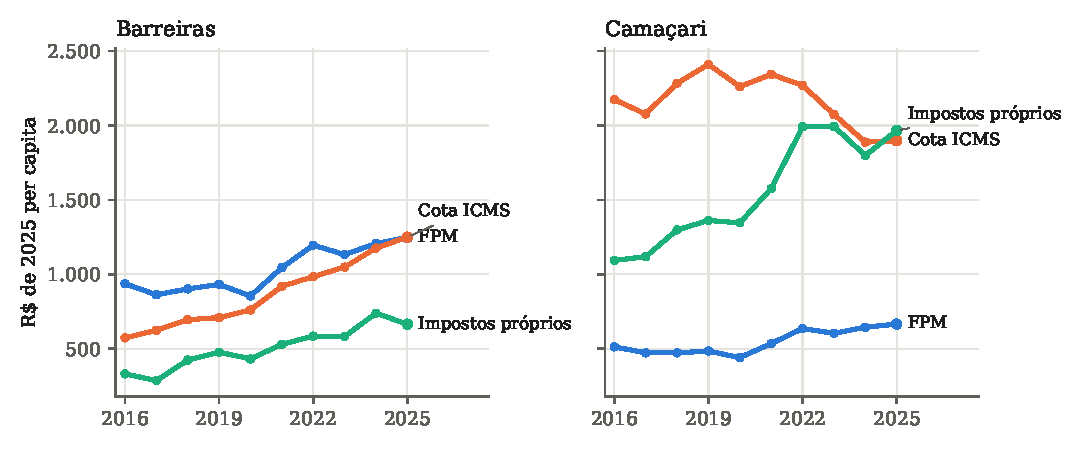
\includegraphics[width=\textwidth]{figuras/fig_fontes_receita.pdf}
  \caption{FPM, cota-parte do ICMS e impostos próprios: valores reais per capita (R\$~de 2025)}
  \label{fig:fontes}
  \fonte{elaboração própria com dados do Siconfi (DCA) e do IBGE.}
\end{figure}

O quadro muda quando a medida se restringe às transferências incondicionais. Em proporção da receita corrente, elas representam de 41\% a 45\% em Barreiras e de 38\% a 48\% em Camaçari nos anos da tabela, e as séries se cruzam: a diferença entre os dois nunca passa de 7 pontos percentuais e muda de sinal no período, com Camaçari acima em 2016 e 2019 e abaixo em 2022 e 2025. A semelhança vale como participação na receita, não em valor: por habitante, Camaçari recebe em média 34\% mais transferências incondicionais (R\$~2.827 contra R\$~2.105). Ela decorre da cota-parte do ICMS, que chegou a 38\% da receita corrente de Camaçari em 2019 e responde, em média, por 77\% de suas transferências incondicionais entre 2016 e 2025, contra 41\% em Barreiras. A hipótese H2 é confirmada para a dependência total e para o FPM, mas não para as transferências incondicionais, em que os municípios se alternam.

Retirada a cota do ICMS, a medida conta outra história (última linha da Tabela~\ref{tab:composicao}). As transferências correntes sem a cota financiam de 24\% a 30\% da receita corrente de Camaçari, contra 59\% a 67\% em Barreiras entre 2016 e 2025, salvo 2017, e a distância entre os dois passa de 15 a 24 para 29 a 40 pontos percentuais. O indicador convencional ordena corretamente o par, mas mais que dobra a dependência de Camaçari em relação a recursos sem vínculo com sua economia, porque conta como transferência uma receita gerada por sua própria indústria. É nesse sentido que a dependência registrada não acompanha a autonomia (H4): ela erra o nível de quem tem a receita vinculada à base local, ainda que acerte a ordem. O resultado é coerente com a conclusão de \citet{Franek2026518} de que a autonomia e a retenção da receita marginal importam mais do que a classificação formal da receita.

A cota do ICMS também acompanha a base local em Barreiras, o que impede tratá-la ali como repasse puramente redistributivo. Entre 2016 e 2025, a cota real per capita do município mais que dobrou, de R\$~573 para R\$~1.249, e em 2025 igualou o FPM por habitante. O movimento pode refletir a expansão do agronegócio no oeste baiano, mas também a parcela da cota repartida por critérios educacionais após a EC n.º 108/2020; o índice de participação publicado pela Secretaria da Fazenda da Bahia permitiria separar os dois efeitos. Em Camaçari, ao contrário, a cota caiu de R\$~2.174 em 2016 para R\$~1.897 em 2025, enquanto os impostos próprios subiram de 19\% para 28\% da receita corrente. A queda tem candidatos óbvios que os dados não permitem separar: o encerramento da produção da Ford no município, em 2021, que reduziu o valor adicionado industrial e, com defasagem, o índice de participação; a limitação do ICMS sobre combustíveis, energia e comunicações, em 2022, que reduziu a arrecadação estadual \citep{LC194}; e as mudanças nos critérios de repartição após a EC n.º 108/2020. A literatura admite duas leituras para a substituição de transferências por arrecadação própria: as duas fontes podem tanto se substituir \citep{DaCosta2016, Taiwo202231} quanto se complementar \citep{Masaki2018173, Porto2023642}. Em Barreiras, os impostos próprios cresceram, mas permanecem em torno de 11\% da receita corrente, o que é compatível com a menor capacidade fiscal do município \citep{dosSantos2017}. A outra face dessa vinculação é distributiva: a regra que devolve o ICMS a quem produz mais dá mais recursos a quem já tem mais base, padrão que a literatura associa às transferências devolutivas \citep{daCosta2024}.

\subsection{Gasto, transferências e PIB: efeitos marginais}

Se a dependência registrada mede mal a autonomia, resta saber se o gasto responde às transferências como prevê o efeito \textit{flypaper}. A Tabela~\ref{tab:regressao} apresenta as estimativas da equação~\eqref{eq:flypaper} em níveis per capita, em que os coeficientes são efeitos marginais em reais. Pelo critério correto da equivalência, o padrão é nítido. Na despesa total (1), cada real adicional de transferência incondicional associa-se a R\$~1,85 de gasto, e cada real adicional de PIB, a um valor estatisticamente nulo ($-$R\$~0,02); a diferença, de R\$~1,87, é significativa ($p = 0{,}014$), com intervalo de confiança de 95\% entre R\$~0,43 e R\$~3,32. Na despesa corrente (2), a diferença é de R\$~1,69 ($p = 0{,}004$). O coeficiente do PIB não se distingue de zero na despesa total, mas é negativo e significativo a 10\% na despesa corrente (2 e 4), e em reais é impreciso: na especificação (1), o intervalo de 95\% para o efeito de um desvio-padrão do PIB per capita (cerca de R\$~11 mil) vai de cerca de $-$R\$~600 a $+$R\$~170. Com $T^{*}$, que exclui a cota do ICMS, os efeitos marginais sobem para cerca de R\$~3 por real (3 e 4), e a diferença em relação ao PIB permanece significativa. A separação entre FPM e ICMS (5) mostra um coeficiente maior para o FPM (R\$~2,94) do que para o ICMS (R\$~0,63), mas a igualdade entre os dois não é rejeitada ($p = 0{,}21$): os dados não sustentam que o gasto responda de modo diferente às duas receitas.

\begin{table}[H]
\centering\footnotesize
\setlength{\tabcolsep}{4pt}
\caption{Gasto municipal, transferências e PIB: efeitos marginais estimados em níveis per capita (2014--2023)}
\label{tab:regressao}
\begin{adjustbox}{max width=\textwidth}
\begin{tabular}{lccccc}
\toprule
 & (1) & (2) & (3) & (4) & (5) \\
\midrule
Variável dependente & $G$ & $G^{c}$ & $G$ & $G^{c}$ & $G^{c}$ \\
\midrule
$T$ (incondicionais) & 1,854** & 1,662*** &  &  &  \\
 & (0,664) & (0,476) &  &  &  \\
$T^{*}$ (sem a cota do ICMS) &  &  & 3,080*** & 2,949*** &  \\
 &  &  & (0,973) & (0,645) &  \\
FPM &  &  &  &  & 2,941*** \\
 &  &  &  &  & (0,975) \\
Cota-parte do ICMS &  &  &  &  & 0,627 \\
 &  &  &  &  & (1,088) \\
$Y$ (PIB) & -0,020 & -0,027* & -0,007 & -0,017* & -0,020 \\
 & (0,016) & (0,015) & (0,010) & (0,008) & (0,013) \\
$D2018$ & 991,752*** & 596,838*** & 1.038,187*** & 627,780*** & 602,511*** \\
 & (247,482) & (158,802) & (258,595) & (164,498) & (174,409) \\
\midrule
Efeito fixo de município & Sim & Sim & Sim & Sim & Sim \\
$\gamma_{\text{transf.}} - \gamma_Y$ & 1,87** & 1,69*** & 3,09*** & 2,97*** & 2,96*** \\
 & (0,68) & (0,49) & (0,98) & (0,65) & (0,98) \\
IC 95\% da diferença & [0,43; 3,32] & [0,65; 2,73] & [1,00; 5,17] & [1,58; 4,35] & [0,87; 5,05] \\
$p$ ($H_0$: FPM = ICMS) & -- & -- & -- & -- & 0,214 \\
Observações & 20 & 20 & 20 & 20 & 20 \\
$R^2$ & 0,895 & 0,935 & 0,898 & 0,945 & 0,942 \\
Durbin-Watson & 1,22 & 0,96 & 1,28 & 1,15 & 1,18 \\
\bottomrule
\end{tabular}
\end{adjustbox}
\par\vspace{3pt}\parbox{\textwidth}{\scriptsize Nota: MQO com efeito fixo de município; variáveis em R\$ de 2025 per capita; erros-padrão robustos HC1 entre parênteses; *** $p<0{,}01$, ** $p<0{,}05$, * $p<0{,}1$. Os coeficientes são efeitos marginais: reais de gasto associados a R\$ 1 a mais da variável. Sob o teorema da equivalência, $\gamma_{\text{transf.}} = \gamma_Y$. $G$ = despesa total; $G^{c}$ = despesa corrente; $T$ = FPM + ITR + cotas de ICMS, IPVA e IPI-exportação + IOF-ouro; $T^{*}$ = $T$ sem a cota do ICMS. Correlação com $Y$ dentro do município: $T$ = 0,72; $T^{*}$ = 0,48; ICMS = 0,78. A cota do ICMS responde, em média, por 78\% das transferências incondicionais de Camaçari e 40\% das de Barreiras (2014--2023). Com 20 observações e erros autocorrelacionados (Durbin-Watson abaixo de 2), os erros-padrão tendem a ser subestimados; os resultados são exploratórios. Fonte: elaboração própria.}
\end{table}


A magnitude dos coeficientes não é implausível por si. Em elasticidade, eles equivalem a cerca de 0,8 para $T$ e 0,5 para $T^{*}$: o gasto cresce menos que proporcionalmente ao recurso, e um efeito de quase três reais por real de $T^{*}$ reflete apenas o fato de $T^{*}$ financiar uma parcela pequena do gasto, que é, em média, seis vezes maior. A dificuldade está em outro ponto. O FPM e as demais transferências seguem o ciclo das finanças federais e estaduais, que move ao mesmo tempo o FUNDEB, as transferências do SUS e a arrecadação própria, e o gasto pode estar acompanhando a receita total. A Seção~\ref{sec:objecao} examina essa possibilidade.

Comparados à literatura brasileira, os resultados ilustram a importância do critério de teste discutido na Seção~\ref{sec:flypaper}. \citet{Paz2020} estimam elasticidade do gasto às transferências de cerca de 0,4 para o conjunto dos municípios e, por ser inferior à unidade, rejeitam o efeito; convertida em efeito marginal, uma elasticidade dessa ordem, com elasticidade ao PIB próxima de zero, é compatível com o fenômeno, como sustentam \citet{Pansani2020}. O fato de a associação aparecer tanto na despesa corrente quanto na total contrasta com \citet{Luz2022}, que encontram o efeito nas despesas de capital financiadas por transferências voluntárias, diferença coerente com o fato de as transferências incondicionais financiarem sobretudo o custeio. O padrão converge com o de \citet{Porto2026}, que, para as províncias argentinas, encontram resposta absoluta maior do gasto corrente que do de capital a choques de transferências.

\subsection{Robustez, placebos e a objeção da cota do ICMS}\label{sec:objecao}

A objeção mais forte aos resultados de base decorre da própria tese do artigo. Se a cota-parte do ICMS acompanha o valor adicionado local, ela não é um recurso externo, e sua inclusão em $T$ aproximaria transferências e PIB, podendo transferir para $\gamma_T$ parte do efeito da renda. Os dados confirmam a premissa: dentro de cada município, a correlação da cota do ICMS com o PIB é de 0,78, e a de $T^{*}$, de 0,48. A objeção, porém, só teria consequência se o PIB tivesse efeito próprio e positivo sobre o gasto, e $\gamma_Y$ não se distingue de zero na maioria das especificações. Retirar a cota não revela um efeito escondido; aumenta o coeficiente da transferência e reduz a colinearidade. E, como a igualdade entre os coeficientes do FPM e do ICMS não é rejeitada, os dados não confirmam a expectativa de que a associação se concentre na receita sem relação com a base local. O que a distinção entre autonomia decisória e vinculação à base local sustenta, nesta amostra, é a leitura descritiva da dependência, e não uma diferença de comportamento do gasto.

\begin{table}[H]
\centering\footnotesize
\setlength{\tabcolsep}{4pt}
\caption{Robustez e placebos: efeito marginal da transferência sobre o gasto (2014--2023)}
\label{tab:robustez}
\begin{adjustbox}{max width=\textwidth}
\begin{tabular}{lcccc}
\toprule
 & \multicolumn{2}{c}{Despesa total ($G$)} & \multicolumn{2}{c}{Despesa corrente ($G^{c}$)} \\
\cmidrule(lr){2-3}\cmidrule(lr){4-5}
Especificação & Coef. (EP) & $p$ & Coef. (EP) & $p$ \\
\midrule
Base: $T^{*}$ (Tabela~\ref{tab:regressao}) & 3,08 (0,97) & 0,007 & 2,95 (0,65) & 0,000 \\
$T$ (com a cota do ICMS) & 1,85 (0,66) & 0,014 & 1,66 (0,48) & 0,004 \\
Sem a dummy $D2018$ & 4,58 (1,70) & 0,017 & 3,86 (1,14) & 0,004 \\
Com tendência linear comum & 3,10 (1,56) & 0,068 & 2,98 (0,98) & 0,009 \\
Sem o ano de 2017 & 2,98 (1,01) & 0,012 & 2,86 (0,66) & 0,001 \\
Sem o ano de 2020 & 4,34 (0,98) & 0,001 & 3,44 (0,75) & 0,001 \\
Sem o ano de 2022 & 3,25 (1,24) & 0,021 & 3,09 (0,83) & 0,003 \\
Totais em log, com ln(população)$^{a}$ & 3,80 (1,70) & 0,043 & 3,94 (0,97) & 0,001 \\
Per capita em log$^{a}$ & 2,80 (1,20) & 0,035 & 3,08 (0,68) & 0,000 \\
Inclinação própria: Camaçari & 5,48 (2,74) & 0,065 & 5,97 (1,53) & 0,002 \\
Inclinação própria: Barreiras & 2,31 (0,96) & 0,031 & 1,99 (0,48) & 0,001 \\
\midrule
Placebo: FUNDEB no lugar de $T^{*}$ & 3,75 (0,98) & 0,002 & 3,23 (0,70) & 0,000 \\
Placebo: SUS no lugar de $T^{*}$ & 1,88 (1,87) & 0,335 & 1,40 (1,54) & 0,378 \\
\bottomrule
\end{tabular}
\end{adjustbox}
\par\vspace{3pt}\parbox{\textwidth}{\scriptsize Nota: cada linha reestima o modelo da Tabela~\ref{tab:regressao} com a alteração indicada; colunas 2--3 para a despesa total ($G$) e 4--5 para a despesa corrente ($G^{c}$). Coef. = reais de gasto por R\$ 1 a mais da transferência indicada (EP HC1); $p$ = teste de igualdade com o efeito marginal do PIB. (a) Efeito marginal calculado pelo método delta a partir das elasticidades (coeficiente $\times$ média do gasto / média da variável). Na especificação com inclinação própria, o $p$ da diferença entre os municípios é 0,304 ($G$) e 0,028 ($G^{c}$). Placebos: o FUNDEB e as transferências do SUS são vinculados, mas acompanham o mesmo ciclo de receitas; um coeficiente semelhante ao de $T^{*}$ indica que a associação não é específica das transferências incondicionais. Fonte: elaboração própria.}
\end{table}


A Tabela~\ref{tab:robustez} reestima o modelo com $T^{*}$ sob várias alterações. A associação resiste à retirada da dummy de 2018, à exclusão de 2017, 2020 ou 2022, à estimação em totais com controle de população e à estimação em logaritmo com efeitos marginais pelo método delta, com diferenças em relação ao PIB significativas ao nível de 5\% em todas essas versões. Com tendência linear comum, a diferença permanece significativa na despesa corrente ($p = 0{,}009$) e fica no limite na despesa total ($p = 0{,}068$). Esses testes mostram que o resultado não depende de um ano atípico nem da forma funcional, mas não tratam do problema central.

O placebo trata dele, e o resultado é desfavorável à interpretação do \textit{flypaper}. Quando o FUNDEB, receita vinculada à educação, substitui $T^{*}$, o gasto total associa-se a R\$~3,75 por real de FUNDEB e o corrente, a R\$~3,23, com diferenças em relação ao PIB significativas ao nível de 1\%: o mesmo padrão, com a mesma magnitude, das transferências incondicionais. Com as transferências do SUS, o coeficiente é positivo, mas impreciso. Como o FUNDEB e as transferências incondicionais crescem juntos, porque ambos acompanham a arrecadação federal e estadual, a associação estimada não é específica das transferências incondicionais. Ela reflete, mais provavelmente, a restrição orçamentária: o gasto acompanha a receita total, e qualquer componente que siga o ciclo comum das receitas parecerá ``grudar''. O placebo, contudo, não é independente: o FUNDEB é formado por 20\% retidos do FPM e das cotas estaduais, de modo que confirma o ciclo comum, mas não o isola. O mesmo diagnóstico decorre da estrutura dos dados, já que, desde 2018, a variação do FPM per capita é a de uma série nacional dividida pela população de cada município.

A especificação com inclinação própria por município parece, à primeira vista, contrariar a expectativa da literatura de efeito maior onde a capacidade fiscal é menor \citep{Saens2026}. Na despesa corrente, o coeficiente de $T^{*}$ é de R\$~5,97 em Camaçari e de R\$~1,99 em Barreiras ($p = 0{,}028$ para a diferença); na despesa total, de R\$~5,48 e R\$~2,31, sem diferença significativa. A diferença, porém, é só de escala: o gasto de Camaçari equivale a quase dez vezes o seu $T^{*}$, e o de Barreiras, a quatro. Convertidos em elasticidade, os coeficientes se igualam: 0,55 em Camaçari e 0,60 em Barreiras na despesa total, e 0,68 e 0,62 na corrente.

Diante disso, a hipótese H1 não é rejeitada, mas também não é confirmada como evidência específica de \textit{flypaper}. Pelo critério correto, o gasto dos dois municípios acompanha as transferências incondicionais muito mais do que o PIB, mas acompanha na mesma medida uma receita vinculada que segue o mesmo ciclo. Com dois municípios e dez anos, o desenho não separa o \textit{flypaper} da resposta do gasto ao ciclo comum das receitas. Testes com descontinuidades do FPM em painéis amplos \citep{Bernardelli2026, Castro2021221} são o caminho para essa separação.

\subsection{Governos locais da Hungria}

Se, no Brasil, a dependência registrada pode esconder autonomia, na Hungria ocorre o inverso. A Tabela~\ref{tab:hungria} e a Figura~\ref{fig:hungria} mostram uma forte contração do setor de governos locais húngaro. A despesa do setor caiu de 9,2\% do PIB em 2012 para 5,4\% em 2025, e sua participação na despesa do governo geral recuou de 18,7\% para 11,3\%. A maior parte da queda ocorreu até 2016, na primeira onda de recentralização descrita por \citet{Dobos2025}, que começou em 2011, antes do início da série. A queda de 2012 para 2013 coincide com a passagem da gestão e do financiamento das escolas para o Estado, ao fim de 2012 \citep{Semjen2023}. Em termos reais per capita, a despesa local oscilou entre cerca de 380 e 530 mil forints de 2025, sem tendência clara: o setor encolheu em relação à economia, não necessariamente em valor absoluto.

\begin{table}[H]
\centering\footnotesize
\setlength{\tabcolsep}{4pt}
\caption{Hungria: tamanho e financiamento dos governos locais (setor S1313)}
\label{tab:hungria}
\begin{adjustbox}{max width=\textwidth}
\begin{tabular}{lrrrrrrr}
\toprule
Indicador & 2012 & 2013 & 2014 & 2016 & 2019 & 2022 & 2025 \\
\midrule
Despesa dos governos locais (\% do PIB) & 9,2 & 7,5 & 7,8 & 5,9 & 6,7 & 5,9 & 5,4 \\
Receita dos governos locais (\% do PIB) & 9,7 & 10,0 & 9,1 & 6,2 & 6,6 & 5,7 & 5,5 \\
Despesa local / desp. do gov. geral & 18,7\% & 15,0\% & 15,6\% & 12,7\% & 14,7\% & 12,1\% & 11,3\% \\
Transf. correntes recebidas (\% do PIB) & 4,6 & 3,0 & 2,9 & 2,5 & 2,1 & 2,1 & 2,0 \\
Transf. de capital recebidas (\% do PIB) & 1,3 & 3,4 & 3,0 & 0,6 & 1,3 & 1,0 & 0,6 \\
Impostos locais (\% do PIB) & 2,4 & 2,2 & 2,1 & 2,2 & 2,1 & 1,7 & 2,0 \\
Transf. correntes / receita sem transf. de capital & 55,5\% & 46,1\% & 47,1\% & 44,6\% & 39,9\% & 44,2\% & 41,2\% \\
Transf. correntes e de capital / receita & 61,7\% & 64,6\% & 64,7\% & 49,5\% & 52,1\% & 54,1\% & 47,1\% \\
Despesa local per capita (mil HUF de 2025) & 475 & 401 & 452 & 383 & 529 & 517 & 492 \\
\bottomrule
\end{tabular}
\end{adjustbox}
\par\vspace{3pt}\parbox{\textwidth}{\scriptsize Nota: governos locais = setor S1313 das contas nacionais (SEC 2010). Transferências correntes = D73 (dentro do governo geral); de capital = D9 (em 2013--2014 inclui a assunção das dívidas municipais pelo governo central); impostos = D2 + D5 + D91. Período: 2012--2025; a série obtida começa já dentro da primeira onda de recentralização. Valores reais deflacionados pelo HICP médio anual (preços de 2025) e divididos pela população (Banco Mundial). Fonte: elaboração própria com dados do Eurostat (gov\_10a\_main, prc\_hicp\_aind) e do Banco Mundial.}
\end{table}


\begin{figure}[H]
  \centering
  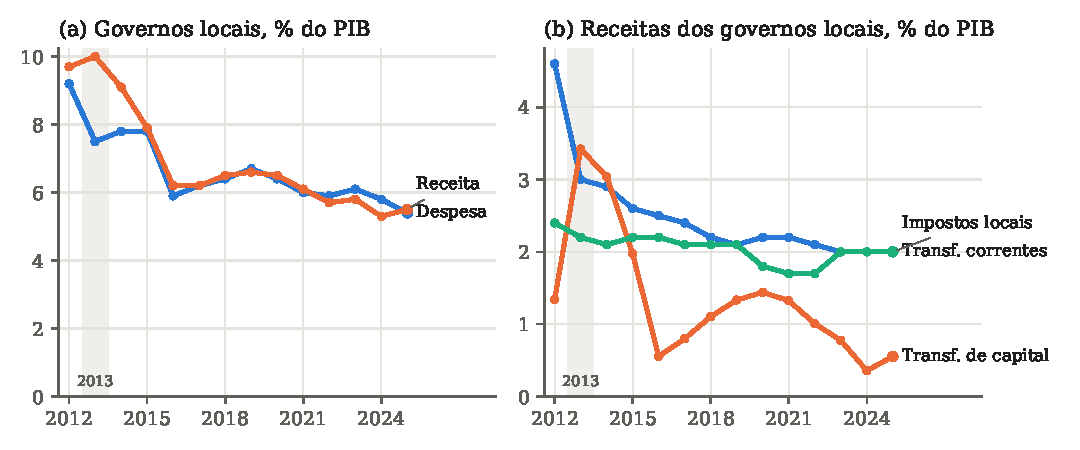
\includegraphics[width=\textwidth]{figuras/fig_hungria_local.pdf}
  \caption{Hungria: tamanho e receitas dos governos locais (2012--2025)}
  \label{fig:hungria}
  \fonte{elaboração própria com dados do Eurostat (gov\_10a\_main). A faixa cinza marca 2013.}
\end{figure}

A leitura do financiamento exige separar as transferências de capital. Em 2013 e 2014, a receita local (10,0\% e 9,1\% do PIB) superou a despesa (7,5\% e 7,8\%), porque o setor recebeu transferências de capital de 3,4\% e 3,0\% do PIB, que correspondem, provavelmente, à assunção das dívidas municipais pelo governo central \citep{Bethlendi2018, Racz202191}. Incluídas essas transferências, a participação das transferências na receita sobe de 61,7\% em 2012 para 64,6\% em 2013 e só depois cai, até 47,1\% em 2025. Em proporção do PIB, o quadro é mais limpo: as transferências correntes recebidas caíram de 4,6\% para 2,0\% do PIB entre 2012 e 2025, enquanto os impostos locais ficaram entre 1,7\% e 2,4\%, apoiados no imposto sobre atividades econômicas \citep{Kecso2020}. Medida sem as transferências de capital no denominador, a participação das transferências correntes caiu de 55,5\% em 2012 para 39\% a 47\% a partir de 2013, sem tendência clara depois de 2019.

A hipótese H3 é, portanto, rejeitada na forma em que foi enunciada, com a ressalva de que ela era teoricamente ambígua. Ao assumir escolas e outros serviços, o Estado deixou de transferir os recursos que os financiavam, e a razão entre transferências e receita caiu porque funções e recursos saíram juntos, ao contrário do caso polonês, em que a recentralização elevou o peso das transferências \citep{Poniatowicz202489}. A literatura sobre a segunda onda indica que o instrumento de controle passou a ser a parcela discricionária das transferências, distribuída segundo o alinhamento político \citep{Vasvari2024467, Vasvari20241371, Kovarek2023}, e os dados agregados do Eurostat não separam essa parcela. Os instrumentos descritos na Seção~\ref{sec:hungria_lit}, o financiamento por tarefa e a contribuição de solidariedade, reduzem o controle local sobre a receita sem aparecer como aumento de dependência, porque o primeiro retira funções e o segundo é uma saída de recursos. O relatório do Índice de Autonomia Local registra a consequência dentro do período da série: a Hungria foi um dos dois únicos países com queda expressiva no escopo de competências locais, quando os escritórios distritais criados em 2013 assumiram parte da assistência social e da educação básica \citep{LAIreport}. Menos dependência veio, assim, acompanhada de menos competências, o que apoia H4 no sentido húngaro. As razões húngaras e brasileiras têm definições diferentes e não são comparáveis em nível; o contraste está na direção dos movimentos, não na comparação dos percentuais.

\subsection{O que mudou em relação ao trabalho anterior}

Os resultados acima dependem de uma base corrigida, e as correções também têm consequências próprias. A atualização partiu do trabalho anterior \citep{DutraP1}, cuja cópia integral foi preservada no repositório. Dos 340 valores municipais comparáveis (17 variáveis, dois municípios, 2014--2023), 327 coincidem com a nova coleta, nove foram corrigidos e quatro, antes ausentes, foram preenchidos. A Tabela~\ref{tab:alteracoes} resume as alterações.

\begin{table}[H]
\centering\footnotesize
\setlength{\tabcolsep}{4pt}
\caption{Principais alterações em relação ao trabalho anterior (2014--2023)}
\label{tab:alteracoes}
\begin{adjustbox}{max width=\textwidth}
\begin{tabular}{p{3.3cm}p{2.1cm}p{6.2cm}r}
\toprule
Variável & Anos & Alteração & Diferença \\
\midrule
Receita total (Camaçari) & 2019--2023 & A base original excluía as receitas intraorçamentárias, mas não as despesas & +1,8 a +5,5\% \\
FPM & Bar. 2016, Cam. 2017 & A base original omitia as parcelas de 1\% & +0,4 a +9,0\% \\
Despesa em saúde (Camaçari) & 2019 & A base original registrava zero; valor da DCA: R\$ 239,3 mi & -- \\
População (Barreiras) & 2018 & Erro de digitação na base original (158.331; IBGE: 153.831) & -2,8\% \\
População & 2022--2023 & Ausente na base original; Censo 2022 e interpolação & -- \\
Resultado orçamentário & 2014--2023 & A base original não descontava a dedução do FUNDEB da receita (R\$ 28 a 158 mi/ano); superávit vira déficit em 7 município-anos (Bar. 2014, Bar. 2015, Bar. 2020, Bar. 2022, Bar. 2023, Cam. 2014, Cam. 2015); ver Tabela~\ref{tab:resultado} & -- \\
Despesa por função & vários & Zeros da base original tratados como ausentes & -- \\
Hungria: receita e despesa do gov. geral & 2014--2021 & A base original trazia estimativas em HUF; a atualização usa o valor oficial do Eurostat & -7,5 a +7,5\% \\
Ampliações & 2014--2025 & 2024--2025; ITR, IPVA, IPI, SUS, deduções do FUNDEB; governos locais húngaros & -- \\
\bottomrule
\end{tabular}
\end{adjustbox}
\par\vspace{3pt}\parbox{\textwidth}{\scriptsize Nota: dos 340 valores municipais comparáveis (17 variáveis, 2 municípios, 2014--2023), 327 coincidem com a base original (diferença menor que 0,1\%). Diferença = (valor novo $-$ valor original)/valor original. Registro completo em data/registro\_alteracoes/. Fonte: elaboração própria.}
\end{table}


A correção de maior consequência é a do resultado orçamentário, detalhada na Tabela~\ref{tab:resultado}. O trabalho anterior o calculou com a receita bruta, sem descontar a dedução para a formação do FUNDEB, de R\$~28 a 158 milhões por ano. Com a correção, o superávit apontado anteriormente vira déficit em sete município-anos entre 2014 e 2023: cinco em Barreiras (2014, 2015, 2020, 2022 e 2023) e dois em Camaçari (2014 e 2015). Somados os anos de 2018 e 2019, já deficitários no cálculo bruto, Barreiras registra resultado de execução negativo em sete dos dez anos de 2014 a 2023. O resultado de um exercício, porém, não mede sozinho a situação fiscal: não considera restos a pagar, disponibilidade de caixa nem superávits financeiros de exercícios anteriores, que podem financiar déficits de execução sem desequilíbrio. A conclusão correta é mais estreita do que ``Barreiras é deficitária'': a leitura de equilíbrio orçamentário persistente do trabalho anterior não se sustenta.

\begin{table}[H]
\centering\footnotesize
\setlength{\tabcolsep}{4pt}
\caption{Resultado orçamentário com e sem a dedução para o FUNDEB (R\$ milhões correntes)}
\label{tab:resultado}
\begin{adjustbox}{max width=\textwidth}
\begin{tabular}{lrrrrrr}
\toprule
 & \multicolumn{3}{c}{Barreiras} & \multicolumn{3}{c}{Camaçari} \\
\cmidrule(lr){2-4}\cmidrule(lr){5-7}
Ano & Bruto & Dedução & Líquido & Bruto & Dedução & Líquido \\
\midrule
2014 & 17,2 & 27,9 & -10,7$^{\dagger}$ & 81,9 & 88,9 & -7,0$^{\dagger}$ \\
2015 & 19,9 & 30,6 & -10,7$^{\dagger}$ & 80,2 & 98,4 & -18,2$^{\dagger}$ \\
2016 & 43,5 & 32,4 & 11,2 & 189,7 & 104,2 & 85,5 \\
2017 & 212,4 & 32,9 & 179,5 & 218,4 & 103,6 & 114,9 \\
2018 & -40,6 & 35,8 & -76,4 & 151,8 & 114,7 & 37,1 \\
2019 & -23,6 & 38,7 & -62,2 & 172,7 & 126,9 & 45,8 \\
2020 & 32,1 & 39,9 & -7,7$^{\dagger}$ & 227,1 & 124,4 & 102,6 \\
2021 & 74,1 & 52,3 & 21,8 & 184,4 & 145,2 & 39,2 \\
2022 & 20,7 & 63,7 & -43,1$^{\dagger}$ & 196,4 & 155,5 & 40,9 \\
2023 & 56,0 & 69,8 & -13,8$^{\dagger}$ & 288,4 & 157,8 & 130,6 \\
2024 & 88,0 & 81,8 & 6,2 & 176,6 & 157,6 & 19,0 \\
2025 & 47,8 & 89,3 & -41,6$^{\dagger}$ & 244,4 & 167,8 & 76,6 \\
\bottomrule
\end{tabular}
\end{adjustbox}
\par\vspace{3pt}\parbox{\textwidth}{\scriptsize Nota: Bruto = receita total bruta menos despesa empenhada, como no trabalho anterior; Líquido = receita total líquida da dedução para a formação do FUNDEB menos despesa empenhada. $\dagger$ = superávit no cálculo bruto que vira déficit no líquido. Entre 2014 e 2023, o resultado líquido é negativo em 7 anos em Barreiras (2014, 2015, 2018, 2019, 2020, 2022, 2023) e em 2 em Camaçari (2014, 2015). O resultado da execução de um exercício não mede, isoladamente, a situação fiscal: não considera restos a pagar, disponibilidade de caixa nem superávits financeiros de exercícios anteriores. Fonte: elaboração própria com dados do Siconfi (DCA).}
\end{table}


Outras correções afetam definições. A receita de Camaçari entre 2019 e 2023 excluía as receitas intraorçamentárias, mas não as despesas correspondentes; o FPM de 2016 e 2017 omitia as parcelas adicionais de 1\%; a despesa em saúde de Camaçari em 2019 aparecia como zero, quando foi de R\$~239,3 milhões; e a população de Barreiras em 2018 tinha dígitos trocados. Para a Hungria, os valores do governo geral em moeda nacional entre 2014 e 2021 eram estimativas, com diferenças de até 7,5\% em relação aos dados oficiais.

A atualização também ampliou a base: incluiu 2024 e 2025, separou as transferências por origem e tipo, incorporou as deduções do FUNDEB e os dados dos governos locais húngaros e substituiu a regressão anterior, que relacionava receita e PIB e juntava municípios de escalas muito diferentes, pelo modelo de efeitos marginais com efeito fixo, testes de robustez e placebos. Um registro merece destaque. Em 2017, Barreiras recebeu R\$~178,6 milhões em ``Outras Transferências Multigovernamentais'', valor que não se repete em nenhum outro ano e equivale a 31,5\% da receita total bruta do exercício, de R\$~567,8 milhões. O valor foi mantido, por ser oficial, mas isolado nas análises de dependência; nas regressões, ele não entra nas transferências incondicionais, e a retirada de 2017 não altera os resultados (Tabela~\ref{tab:robustez}). Sua natureza não foi confirmada em fonte primária e merece verificação.

\section{CONCLUSÃO}\label{sec:conclusao}

A principal conclusão deste artigo é que a dependência de transferências, como a contabilidade a registra, não acompanha a autonomia fiscal. O indicador ordena corretamente os municípios, mas erra o nível de quem tem a receita vinculada à própria economia, e pode cair enquanto a autonomia cai. O que importa é quem controla a receita e de onde ela vem, não o rótulo que ela recebe no orçamento, e é por isso que índices de autonomia mais completos medem essas dimensões em separado \citep{Ladner2016}.

Em Camaçari, boa parte da ``dependência'' é a própria economia do município voltando ao caixa da prefeitura pela cota do ICMS. No papel, mais da metade de sua receita vem de transferências; sem a cota, menos de um terço. O município não controla essa base, mas também não depende de decisões alheias para recebê-la: está vinculado à própria economia, para o bem e para o mal, como mostrou a saída da Ford. Barreiras, ao contrário, depende de fato de decisões tomadas fora, porque o FPM segue a arrecadação federal. Essa vinculação tem um custo distributivo: ao devolver o ICMS a quem produz mais, a regra concentra recursos onde já há riqueza \citep{daCosta2024}. Vinculação à base e redistribuição puxam em sentidos opostos, e a reforma tributária, ao repartir o futuro IBS sobretudo pela população \citep{EC132}, escolhe a redistribuição: tende a desligar a receita dos municípios industriais de sua própria economia e a dar mais recursos aos demais.

A Hungria mostra o caminho inverso, com menos dependência e menos autonomia: pelos instrumentos descritos na Seção~\ref{sec:hungria_lit}, o governo central reduziu o controle local sobre funções e receitas sem que isso aparecesse como aumento do peso das transferências. Não há paradoxo nisso, porque funções e recursos saíram juntos; há apenas um indicador que não foi feito para captar controle.

Quanto ao efeito \textit{flypaper}, o gasto dos dois municípios acompanha as transferências muito mais do que o PIB, mas acompanha na mesma medida o FUNDEB, e com dois municípios não é possível separar o efeito da regra de gastar o que se arrecada. Assim, H1 fica sem confirmação; H2 vale para a dependência total, mas não para as transferências incondicionais; H3 é rejeitada; e H4 recebe apoio descritivo nos dois países.

O estudo contribui com uma base de dados aberta e corrigida, que revelou, entre outros pontos, resultados orçamentários negativos em Barreiras antes registrados como superávits, e com um alerta para quem avalia finanças municipais: indicadores de autonomia precisam separar a receita que nasce da economia local da que vem de fora. Com dois municípios, as conclusões não se generalizam nem identificam causas. Um painel com os municípios do interior na faixa máxima do FPM \citep{Bernardelli2026, Castro2021221} e dados municipais sobre as transferências discricionárias na Hungria são os próximos passos naturais.


% ========================== referências
% Artigos de periódicos (mínimo 80, citados e discutidos) + documentos, bases, legislação, P1 e tese.
\bibliographystyle{plainnat-pt}
\clearpage\phantomsection\addcontentsline{toc}{section}{REFERÊNCIAS}
\begingroup
\small\singlespacing
\setlength{\bibsep}{3pt plus 1pt}
\bibliography{referencias,candidatas}
\endgroup

\end{document}
